\chapter{Proof of Concept}
\label{sec:proof_of_concept}

% -------------------------------------------------------------------------------

% parameers: xlabel, center
\newcommand{\fuzzyTreeNode}[2]{
    \begin{tikzpicture}
        \begin{axis}%
            [
                title = {Fuzzy Split: $#1 \leq #2$},
                width=4.5cm,
                height=3cm,
                axis lines=center,
                xlabel={#1},
                x label style={at={(axis description cs:0.9,-0.1)},anchor=north},
                ylabel=$\mu$,
                y label style={at={(axis description cs:0.5,1)},anchor=south},
                xmin=-5,
                xmax=5,
                xtick={},
                xticklabels= {},
                ytick={},
                yticklabels={},
                extra x ticks={0},
                extra x tick labels={#2},
                ymax=1,
                samples=50,
                extra y ticks={1},
                every axis plot/.append style={thick}
            ]
            \addplot[red]  {sigmoid(x,0,-1)};
            \addplot[blue] {sigmoid(x,0,1)};
            \node[anchor=center, red] at (axis cs:-2.9,0.6) {$\mu_{\text{#1smaller#2}}$};
            \node[anchor=center, blue] at (axis cs:3.1,0.6) {$\mu_{\text{#1greater#2}}$};
        \end{axis}

    \end{tikzpicture}
}

\newcommand{\fuzzyTreeLeaf}[1]{
    \begin{tikzpicture}
        \begin{axis}%
            [
                title = {Class: #1},
                width=3.25cm,
                height=2.25cm,
                axis lines=center,
                xlabel={$\text{class}$},
                x label style={at={(axis description cs:0.6,-0.3)},anchor=west},
                ylabel=$\mu$,
                y label style={at={(axis description cs:0.5,1)},anchor=south},
                xmin=-5,
                xmax=5,
                xtick={},
                xticklabels= {},
                ytick={},
                yticklabels={},
                extra x ticks={0},
                extra x tick labels={#1},
                ymax=1,
                samples=10,
                extra y ticks={1},
                every axis plot/.append style={thick}
            ]
            \addplot[black]  {gaussian(x,0,1)};
        \end{axis}

    \end{tikzpicture}
}

% parameers: xlabel, center
\newcommand{\crispTreeNode}[2]{
    \begin{tikzpicture}
        \begin{axis}%
            [
                title = {Crisp Split: $#1 \leq #2$},
                width=4.5cm,
                height=3cm,
                axis lines=center,
                xlabel={#1},
                x label style={at={(axis description cs:0.9,-0.1)},anchor=north},
                ylabel=$\mu$,
                y label style={at={(axis description cs:0.5,1)},anchor=south},
                xmin=-5,
                xmax=5,
                xtick={},
                xticklabels= {},
                ytick={},
                yticklabels={},
                extra x ticks={0},
                extra x tick labels={#2},
                ymin=-0.1,
                ymax=1.1,
                samples=50,
                extra y ticks={1},
                every axis plot/.append style={thick}
            ]
            \addplot[red,domain=-5:-0.6] {step(x,0,-1)};
            \addplot[blue,domain=0.6:5] {step(x,0,1)};
            \addplot[red,domain=0.6:5] {step(x,0,-1)};
            \addplot[blue,domain=-5:-0.6] {step(x,0,1)};

            \node[draw,draw=black,circle,inner sep=1pt,minimum width=3pt,thick] at (axis cs:0,1) {};
            \node[draw,draw=black,circle,inner sep=1pt,minimum width=3pt,thick] at (axis cs:0,0) {};

            \node[anchor=center, red] at (axis cs:-2.9,0.6) {$#1 \leq #2$};
            \node[anchor=center, blue] at (axis cs:3.1,0.6) {$#1 > #2$};
        \end{axis}

    \end{tikzpicture}
}


% -------------------------------------------------------------------------------

This chapter presents a proof of concept for the fuzzy tuning technique. We will develop two different knowledge bases to predict the optimal configurations for \texttt{\gls{mdflexible}} simulations.

Creating the knowledge base is one of the most complex parts of developing a fuzzy system, as it typically requires a profound understanding of the system to create meaningful rules, which may be difficult to obtain. Luckily, methods such as data-driven approaches exist to semi-automate this process. Such data-driven methods do not require prior expert knowledge about the system and provide a good initial set of rules that can be further refined by experts if desired.

In this work, we will use a decision tree approach proposed by Crockett et al.~\cite{CROCKETT20062809}. This proposed method uses machine learning to first train decision trees on the dataset to create an initial crisp rule base. In the second step, the decision trees are converted into so-called fuzzy decision trees, which can then be used to extract the linguistic variables and fuzzy rules.

\section{Data Driven Rule Extraction}

\subsection{Decision Trees}

Decision trees are prevalent machine learning algorithms used for classification and regression tasks. They work by recursively partitioning the input using axis-parallel splits so that the resulting subsets are as pure as possible. Concretely, they try to minimize a given impurity metric, such as the Gini impurity $I_G = \sum_{i=1}^{n} p_i(1-p_i)$ of the subsets~\cite{10.5555/2380985}. The probability $p_i$ is the fraction of samples in the subset that belong to class $i$, and $n$ is the total number of classes.

Since decision trees directly partition the input space into regions with different classes, they can also be depicted using their decision surface if the dimensionality allows it. The decision surface of a decision tree is a piecewise constant function that assigns the predicted class label to each point in the input space of the decision tree. An example decision tree and its decision surface are shown in \autoref{fig:decisionTreeExample} and \autoref{fig:decisionBoundaryExample}.

% Image of a decision tree
\begin{multicols}{2}
    \begin{figure}[H] % [H] for HERE
        \centering
        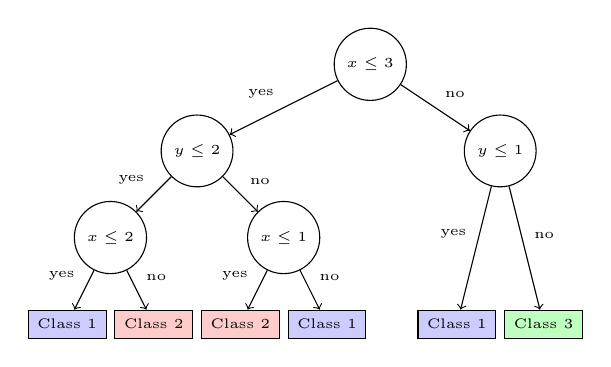
\begin{tikzpicture}[scale=1.1,font=\tiny]
            \node [circle, draw] (A) at (0,0) {$x \leq 3$};
            \node [circle, draw] (B) at (-2,-1) {$y \leq 2$};
            \node [circle, draw] (C) at (1.5,-1) {$y \leq 1$};
            \node [circle, draw] (D) at (-3,-2) {$x \leq 2$};
            \node [circle, draw] (E) at (-1,-2) {$x \leq 1$};

            \node [rectangle,draw,fill=blue!20] (F) at (-3.5,-3) {Class 1};
            \node [rectangle,draw,fill=red!20] (G) at (-2.5,-3) {Class 2};
            \node [rectangle,draw,fill=red!20] (H) at (-1.5,-3) {Class 2};
            \node [rectangle,draw,fill=blue!20] (I) at (-0.5,-3) {Class 1};
            \node [rectangle,draw,fill=blue!20] (J) at (1,-3) {Class 1};
            \node [rectangle,draw,fill=green!25] (K) at (2,-3) {Class 3};

            \draw[->] (A) -- (B) node [midway, left, above left] {yes};
            \draw[->] (A) -- (C) node [midway, right, above right] {no};
            \draw[->] (B) -- (D) node [midway, left, above left] {yes};
            \draw[->] (B) -- (E) node [midway, right, above right] {no};

            \draw[->] (C) -- (J) node [midway, left, above left] {yes};
            \draw[->] (C) -- (K) node [midway, right, above right] {no};

            \draw[->] (D) -- (F) node [midway, left, above left] {yes};
            \draw[->] (D) -- (G) node [midway, right, above right] {no};

            \draw[->] (E) -- (H) node [midway, left, above left] {yes};
            \draw[->] (E) -- (I) node [midway, right, above right] {no};

        \end{tikzpicture}

        \caption[Decision tree used for the example]{An example decision tree for a dataset with two features $x$ and $y$. There are three distinct classes in the dataset}
        \label{fig:decisionTreeExample}
    \end{figure}

    \columnbreak    % start next column

    \begin{figure}[H]
        \centering
        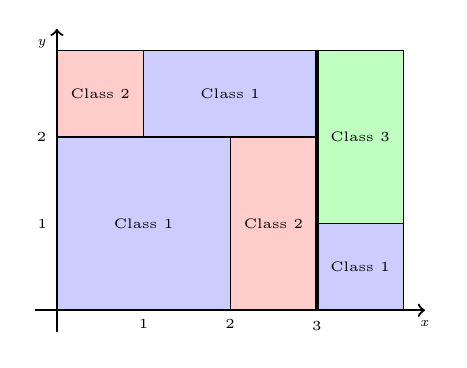
\begin{tikzpicture}[scale=1.1,font=\tiny]

            \draw[fill=red!20] (0,2) -- (1,2) -- (1,3) -- (0,3) -- cycle;

            \draw[fill=blue!20] (1,2) -- (3,2) -- (3,3) -- (1,3) -- cycle;

            \draw[fill=blue!20] (0,0) -- (2,0) -- (2,2) -- (0,2) -- cycle;
            \draw[fill=red!20] (2,0) -- (3,0) -- (3,2) -- (2,2) -- cycle;

            \draw[fill=blue!20] (3,0) -- (4,0) -- (4,1) -- (3,1) -- cycle;
            \draw[fill=green!25] (3,1) -- (4,1) -- (4,3) -- (3,3) -- cycle;

            \draw[->, thick] (-0.25,0) -- (4.25,0) node [below] {\textit{x}};
            \draw[->, thick] (0,-0.25) -- (0,3.25) node [below left] {\textit{y}};

            % decision lines

            \draw[line width=1.5pt,] (3,0) node [below] {3}  -- (3,3) ;
            \draw[line width=1pt] (0,2) node [left] {2} -- (3,2);

            \draw[] (2,0) node [below] {2}-- (2,2);

            \node [below] at (1,0) {1};

            \node [left] at (0,1) {1};

            % area labels
            \node [] at (0.5,2.5) {Class 2};
            \node [] at (2,2.5) {Class 1};

            \node [] at (1,1) {Class 1};
            \node [] at (2.5,1) {Class 2};


            \node [] at (3.5,2) {Class 3};
            \node [] at (3.5,0.5) {Class 1};

        \end{tikzpicture}
        \caption[Decision surface of the example decision tree]{The decision surface of the decision tree from \autoref{fig:decisionTreeExample} on $\mathcal{D}=[0,4]\times[0,3]$. }
        \label{fig:decisionBoundaryExample}
    \end{figure}
\end{multicols}


\subsection{Conversion of Decision Trees to Fuzzy Systems}

This section will demonstrate how to convert a classical decision tree into a fuzzy decision system using the fictional decision tree from \autoref{fig:decisionTreeExample} as an example.

\subsubsection{Fuzzy Decision Trees}

As the conversion makes use of so-called fuzzy decision trees, we will briefly introduce them here. Fuzzy decision trees are a generalization of classical decision trees and allow for fuzzy logic to be used in the decision-making process. Instead of following the classical \texttt{if then else} logic to descend into the decision tree, it uses fuzzy sets at each node of the tree to fuzzily calculate the contribution of each branch to the final decision based on the degree of truth of both possible paths. Contrary to classical decision trees, which follow a single path from the root to a leaf node, fuzzy decision trees explore all possible paths simultaneously and make a final decision by aggregating the results of the paths using fuzzy logic operations.

\subsubsection{Conversion}


A classical decision tree is converted into a fuzzy decision tree by replacing the crisp decision (e.g., $x \leq 3$) at each internal node of the decision tree with a fuzzy set. Those fuzzy sets should maintain the same semantics as the crisp decision but should provide a continuous value in the range $[0,1]$ specifying the degree of how much each branch should be considered. Classical decision trees can only make binary decisions (${0,1}$), which causes them to only consider a single path of the decision tree. Allowing them to consider multiple paths simultaneously can drastically increase the decision-making capabilities of the decision tree, especially in boundary cases where the decision can be ambiguous.


The shape of the membership functions of the fuzzy sets can be chosen arbitrarily, but since trees work with one-sided boundaries, typical choices include complementary \texttt{sigmoid}-shaped functions that are centered around the crisp decision boundary (See \autoref{fig:fuzzyMembershipFunctions}), as those function shapes maintain the semantics of the branching idea. Crockett et al.~\cite{CROCKETT20062809} suggested creating those sigmoid shapes with a \emph{width} proportional to the standard deviation of the attribute. In Particular, the authors suggested an interval $[t-n\cdot \sigma, t+n\cdot \sigma]$ for the membership function, where  $t$ is the value of the decision boundary, $\sigma$ is the standard deviation of the attribute and $n$ is a parameter that can be adjusted to control the \emph{width} of the membership function. This interval specifies the region of the membership function where most of the change in membership occurs. The value of $n$ is typically chosen from the interval $n\in [0,5]$ as the membership function can become too broad otherwise and could even weaken the decision-making process~\cite{CROCKETT20062809}. In this work, we will use $n=2$ as a default value. Using this method, it is possible to fully automate the conversion of a decision tree into a fuzzy decision tree, which we will utilize in this work.


\begin{figure}[h]
    \centering
    \begin{tikzpicture}[scale=2,font=\tiny]
        \node [rectangle,rounded corners,draw,inner sep=2pt] (A) at (0.5,0) {
            \crispTreeNode{x}{3}
        };

        \node [rectangle,rounded corners,draw,inner sep=2pt] (B) at (3.5,0) {
            \fuzzyTreeNode{x}{3}
        };

        \path[draw=black, line width=1mm, -{Triangle[length=4mm, bend]}]
        (1.5,0) to [bend left] (2.5,0);

        \path[draw=white, line width=0.5mm, -{Triangle[length=3.25mm, bend, angle'=60]}, shorten >= 0.5mm, shorten <= 0.25mm]
        (1.5,0) to [bend left] (2.5,0);

    \end{tikzpicture}
    \caption[Conversion of crisp tree node into fuzzy tree node]{Conversion of crisp set membership functions to fuzzy set membership functions. The classical membership functions $x \leq 3$ and $x>3$ of a decision tree node are replaced by two \texttt{sigmoid}-shaped membership functions \textcolor{red}{$\mu_{\text{xsmaller3}}$} and \textcolor{blue}{$\mu_{\text{xgreater3}}$} that specify to which degree one should traverse left or right. The \emph{width} of the membership functions is data dependent and is set to $n\cdot \sigma = 2 \cdot \sigma$. }
    \label{fig:fuzzyMembershipFunctions}
\end{figure}

Once the internal nodes of the decision tree have been converted, the next step is to convert the leaf nodes of the decision tree to fuzzy leaf nodes. As the outputs of decision trees are specific class labels, we can define a single linguistic variable consisting of all possible class labels together with a corresponding fuzzy set. The shapes of the membership functions for the fuzzy sets can again be chosen mostly arbitrarily, but we will use \texttt{gaussian} functions with a different mean as they are a good choice for representing class labels in a continuous domain. This way of placing the fuzzy sets is not directly obvious, and the placement can significantly influence the defuzzification process depending on the chosen defuzzification function, as we will see later. However, we can minimize this issue by carefully choosing a suitable defuzzification method.
The resulting conversion of the decision tree in \autoref{fig:decisionTreeExample} into a fuzzy decision tree is shown in \autoref{fig:fuzzyDecisionTreeExample}.


\begin{figure}[h!]
    \centering
    \begin{tikzpicture}[scale=1.9,font=\tiny]

        \node [rectangle, rounded corners, draw, inner sep=2pt] (A) at (0,0) {
            \fuzzyTreeNode{x}{3}
        };

        \node [rectangle,rounded corners,draw,inner sep=2pt] (B) at (-2,-1.6) {
            \fuzzyTreeNode{y}{2}
        };

        \node [rectangle,rounded corners,draw,inner sep=2pt] (C) at (1.8,-1.6) {
            \fuzzyTreeNode{y}{1}
        };

        \node [rectangle,rounded corners,draw,inner sep=2pt] (D) at (-3,-3.2) {
            \fuzzyTreeNode{x}{2}
        };

        \node [rectangle,rounded corners,draw,inner sep=2pt] (E) at (-1,-3.2) {
            \fuzzyTreeNode{x}{1}
        };


        \node [rectangle,rounded corners,draw,inner sep=2pt,fill=blue!20] (F) at (-3.7,-4.7) {
            \fuzzyTreeLeaf{1}
        };

        \node [rectangle,rounded corners,draw,inner sep=2pt,fill=orange!20] (G) at (-2.6,-4.7) {
            \fuzzyTreeLeaf{2}
        };

        \node [rectangle,rounded corners,draw,inner sep=2pt,fill=orange!20] (H) at (-1.5,-4.7) {
            \fuzzyTreeLeaf{2}
        };

        \node [rectangle,rounded corners,draw,inner sep=2pt,fill=blue!20] (I) at (-0.4,-4.7) {
            \fuzzyTreeLeaf{1}
        };

        \node [rectangle,rounded corners,draw,inner sep=2pt,fill=blue!20] (J) at (1.25,-4.7) {
            \fuzzyTreeLeaf{1}
        };

        \node [rectangle,rounded corners,draw,inner sep=2pt,fill=green!20] (K) at (2.35,-4.7) {
            \fuzzyTreeLeaf{3}
        };



        \draw[->] (A) -- (B) node [pos=.4, left, above left] {yes};
        \draw[->] (A) -- (C) node [pos=.4, right, above right] {no};

        \draw[->] (B) -- (D) node [pos=.8, left, above left] {yes};
        \draw[->] (B) -- (E) node [pos=.8, right, above right] {no};

        \draw[->] (C) -- (J) node [pos=.2, left, above left] {yes};
        \draw[->] (C) -- (K) node [pos=.2, right, above right] {no};

        \draw[->] (D) -- (F) node [pos=.6, left, above left] {yes};
        \draw[->] (D) -- (G) node [pos=.6, right, above right] {no};

        \draw[->] (E) -- (H) node [pos=.6, left, above left] {yes};
        \draw[->] (E) -- (I) node [pos=.6, right, above right] {no};
    \end{tikzpicture}

    \caption[Fuzzy decision tree created from the regular decision tree]{The fuzzy decision tree corresponding to the decision tree in \autoref{fig:decisionTreeExample}. Internal nodes use two \texttt{sigmoid} membership functions (\textcolor{red}{$\mu_{\text{smaller}}$} and \textcolor{blue}{$\mu_{\text{greater}}$}) instead of a crisp decision. The leaf nodes use different \texttt{gaussian} membership functions centered around a unique mean.}

    \label{fig:fuzzyDecisionTreeExample}
\end{figure}

It is now possible to fully extract all linguistic variables from the fuzzy decision tree. Every fuzzy set defined over the same variable can be collected into a single linguistic variable. This results in linguistic variables consisting of a bunch of different \texttt{sigmoid} membership functions for input variables (internal nodes) and a single linguistic variable with different \texttt{gaussian} membership functions for the output variable (leaf nodes). The resulting linguistic variables are shown in \autoref{fig:fuzzyDecisionTreeLinguisticVariables}.


\begin{figure}[h]
    \centering

    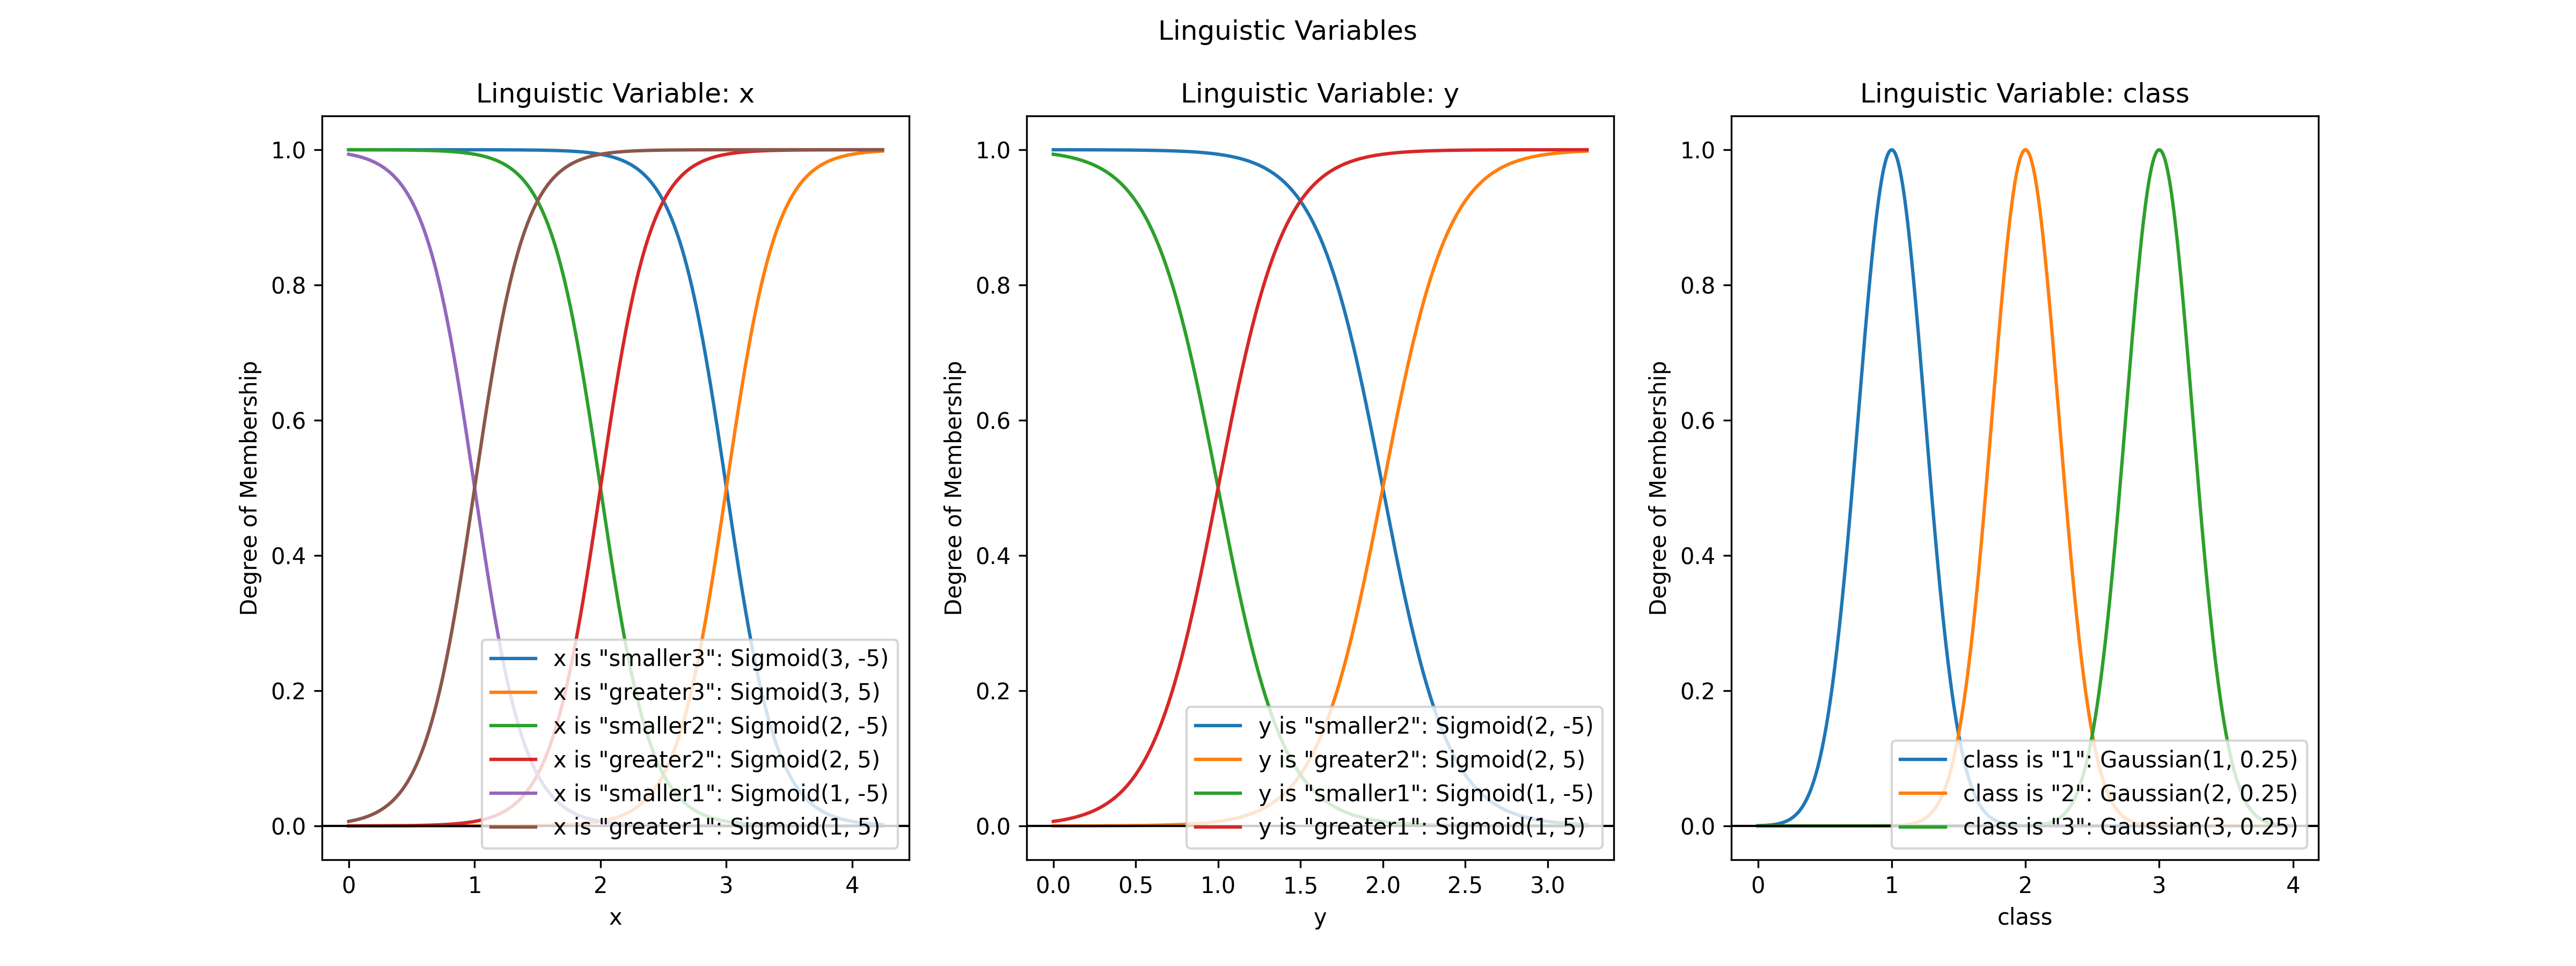
\includegraphics[width=\linewidth]{figures/ProofOfConcepts/fuzzy_sets.png}

    \caption[Linguistic variables for the converted fuzzy decision tree]{Linguistic variables used in the fuzzy decision tree of \autoref{fig:fuzzyDecisionTreeExample}. The standard deviation of the attributes is assumed to be $\sigma \approx 0.5$ such that the \emph{width} of the sigmoid membership functions is $n\cdot \sigma \approx 1$. The standard deviation of the class values is chosen so that they do not overlap too much.}
    \label{fig:fuzzyDecisionTreeLinguisticVariables}
\end{figure}

\subsubsection{Rule Extraction}

The final step is to extract the fuzzy rules from the tree. This can be done by traversing the tree in a depth-first manner and collecting the correct membership functions for each path ending in a leaf node along the way. As all conditions of this path have to hold simultaneously, all fuzzy sets are connected using the \texttt{AND} operation. This newly created fuzzy set, which consists of the intersection of all fuzzy sets along the way, is the premise of selecting the fuzzy set of the leaf node. Consequently, both fuzzy sets are connected using the Mamdani \texttt{IMPLICATION} operator. This implication then forms a rule for the fuzzy system. Therefore, each unique path traversing the tree results in a unique rule. This process essentially mimics the decision surface seen in \autoref{fig:decisionBoundaryExample}, as we create precisely one rule for each region of the decision surface. The rules extracted from the fuzzy decision tree in \autoref{fig:fuzzyDecisionTreeExample} using this method are shown in \autoref{tab:fuzzyRulesExample}.


\newpage
\newcommand{\is}{\textit{ is }}


\begin{table}[H]
    \centering
    \begin{tabular}{c|l|c}
        \textbf{Rule} & \textbf{Antecedent}                                                             & \textbf{Consequent} \\
        \hline
        1             & $x \is \text{smaller3} \land y \is \text{smaller2} \land x \is \text{smaller2}$ & $class \is 1$       \\
        2             & $x \is \text{smaller3} \land y \is \text{smaller2} \land x \is \text{greater2}$ & $class \is 2$       \\
        3             & $x \is \text{smaller3} \land y \is \text{greater2} \land x \is \text{smaller1}$ & $class \is 2$       \\
        4             & $x \is \text{smaller3} \land y \is \text{greater2} \land x \is \text{greater1}$ & $class \is 1$       \\
        5             & $x \is \text{greater3} \land y \is \text{smaller1}$                             & $class \is 1$       \\
        6             & $x \is \text{greater3} \land y \is \text{greater1}$                             & $class \is 3$       \\
    \end{tabular}
    \caption[Extracted fuzzy rules from the fuzzy decision tree]{Extracted fuzzy rules from the fuzzy decision tree in \autoref{fig:fuzzyDecisionTreeExample} in the format: $\textbf{IF} \text{ Antecedent } \textbf{THEN} \text{ Consequent }$}
    \label{tab:fuzzyRulesExample}
\end{table}

\subsubsection{Fuzzy System}

With the linguistic variables and fuzzy rules extracted from the decision tree, we can finally use them to create a fuzzy system that can predict the class of a new data point based on its features. Since the fuzzy system can be seen as a black box mapping continuous input features to continuous output classes, we represent them as shown in \autoref{fig:fuzzySystem} from now on. It is also possible to visualize the fuzzy system's decision surface by evaluating the system for each point in the input space, as shown in \autoref{fig:fuzzyDecisionSurfaceComparison} for two different defuzzification methods. Such visualizations can help understand the decision-making process of the fuzzy system but, unfortunately, are not possible for higher-dimensional input spaces.


\begin{figure}[h]
    \centering
    \begin{tikzpicture}[scale=2,font=\small]

        \node [rectangle,rounded corners,draw,inner sep=2pt] (B) at (0,1.2) {
            Rules, Linguistic Variables \& Defuzzification Method
        };


        \node [rectangle, rounded corners, draw, inner sep=2pt,fill=white!80!black, fill ] (A) at (0,0) {
            \begin{tikzpicture}[scale=2,font=\tiny]
                \begin{axis}%
                    [
                        title={FCS},
                        width=3cm,
                        height=2cm,
                        axis lines=center,
                        xmin=0,
                        xmax=4,
                        xlabel={$\mathbb{R}$},
                        x label style={at={(axis description cs:1,0.2)},anchor=west},
                        ylabel=$\mu$,
                        y label style={at={(axis description cs:0,0.8)},anchor=east},
                        xtick={},
                        xticklabels= {},
                        ytick={},
                        yticklabels={},
                        ymax=1,
                        every axis plot/.append style={thick},
                        domain=0:4
                    ]
                    \addplot[blue, samples=17] {gaussian(x,1,0.2)};
                    \addplot[red,samples=15] {gaussian(x,2,0.2)};
                    \addplot[green,samples=17] {gaussian(x,3,0.2)};
                \end{axis}
            \end{tikzpicture}
        };



        \draw[->,thick] (B) -- (A);

        \draw[->,ultra thick] (-2.5,+0.2) -- (A) node [left, pos=0] {$x \in \mathbb{R}$};
        \draw[->,ultra thick] (-2.5,-0.2) -- (A) node [left, pos=0] {$y \in \mathbb{R}$};
        \draw[->,ultra thick] (A) -- (2.5,0) node [right, pos=1] {$class \in \mathbb{R}$};
    \end{tikzpicture}

    \caption[Fuzzy system created from the fuzzy decision tree seen as a black box]{The fuzzy system created from the fuzzy decision tree in \autoref{fig:fuzzyDecisionTreeExample} can be seen as a black box that maps continuous input features to continuous output classes.}

    \label{fig:fuzzySystem}
\end{figure}

\subsubsection{Choice of Defuzzification Method}

The exact shape of the decision surface depends on the specific defuzzification method used. The most common choice in literature is the \gls{cog} method, which calculates the $x$-position of the center of gravity of the membership function of the final fuzzy set.
However, using the \gls{cog} method can lead to undesired results when using nominal values for the output classes, which we will see later. The main problem is that the values have no concept of order. Without such an ordering, the interpolation between the different classes performed by methods such as \gls{cog} is not meaningful and leads to wrong predictions. Other methods, such as the \gls{mom} method, can be used instead. This method calculates the mean value of the maximum membership functions. In most cases, this method will return precisely the center of the membership function with the highest value and is a good choice for such types of knowledge bases. A direct comparison of the two methods on a critical datapoint is shown in \autoref{fig:fuzzySetForDataCOG} and \autoref{fig:fuzzySetForDataMOM}. Using the \gls{cog} method results in an opposite class than originally predicted from the fuzzy system, while the \gls{mom} method correctly predicts the class.

\begin{figure}
    \centering
    \begin{subfigure}[t]{0.48\textwidth}
        \centering
        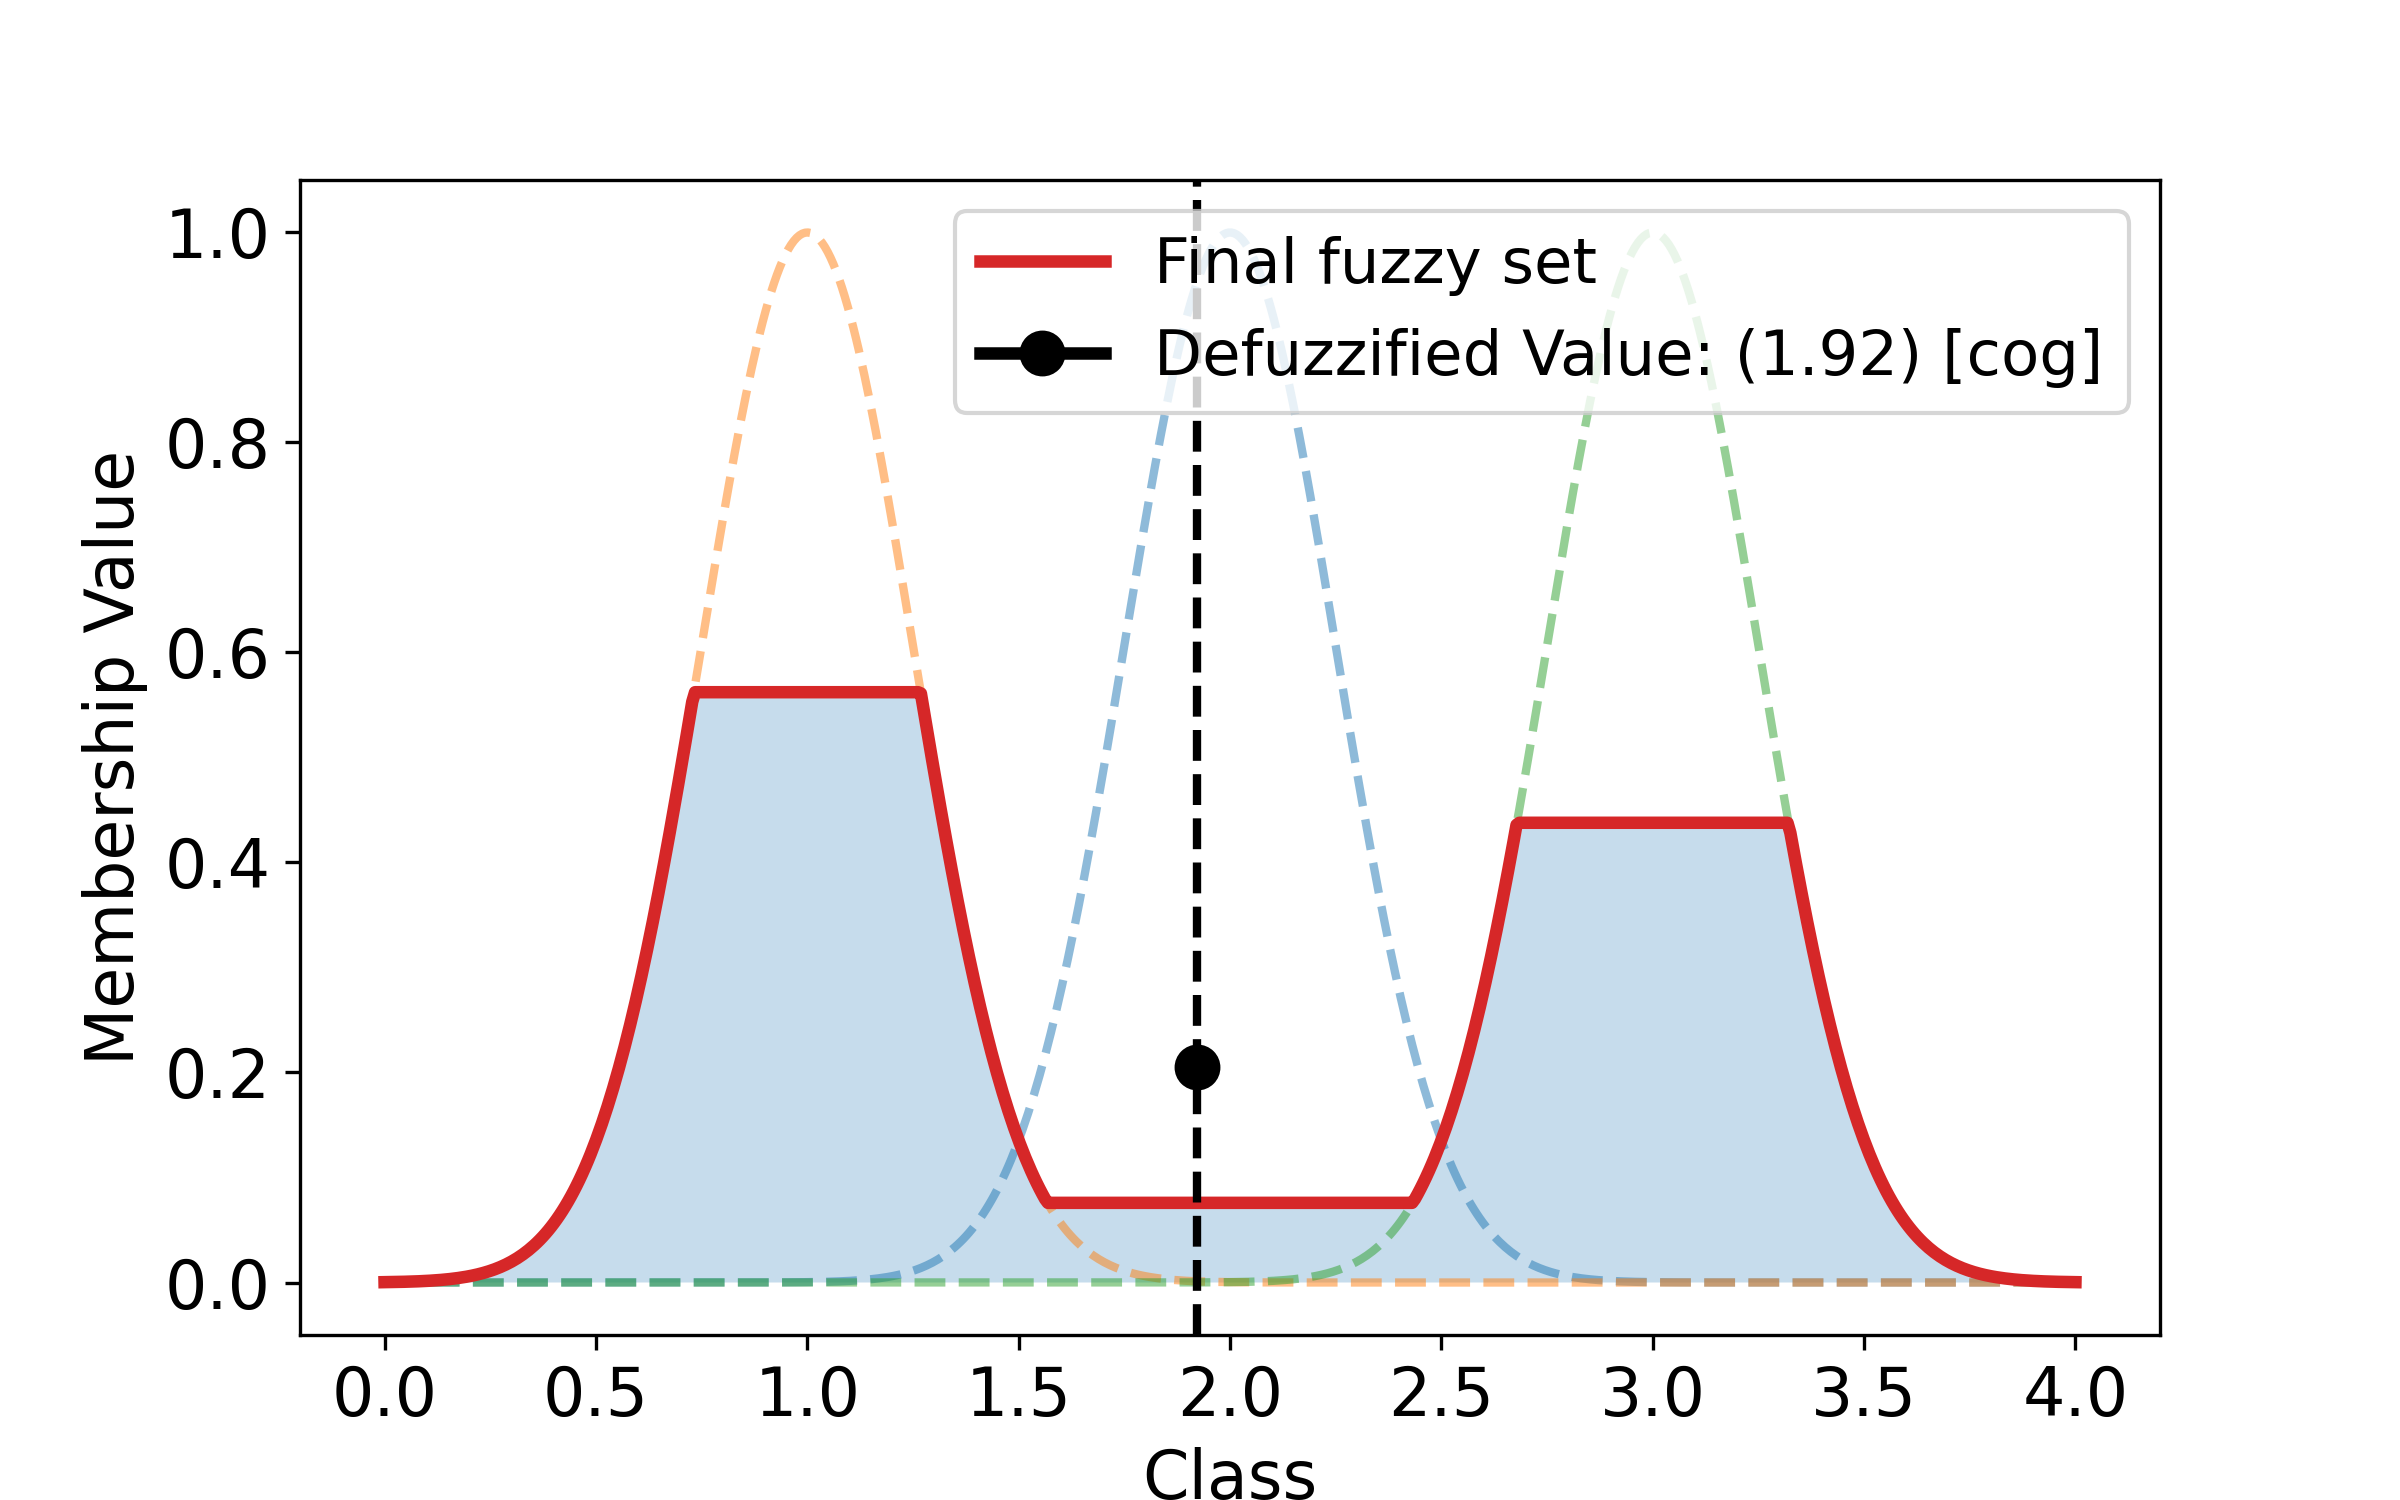
\includegraphics[width=\textwidth,trim={0 0 0 1cm},clip]{figures/ProofOfConcepts/fuzzy_set_for_data_cog.png}
        \caption[Resulting Fuzzy Set after applying the Rules on specific Data, COG Method]{Defuzzification on the fuzzy obtained by applying the rules from \autoref{tab:fuzzyRulesExample} on the data point $(x=2.95, y=2.5)$. There are clear peaks at the class values 1 and 3. However, the \gls{cog} method incorrectly suggests values close to class 2.}
        \label{fig:fuzzySetForDataCOG}
    \end{subfigure}
    \hfill
    \begin{subfigure}[t]{0.48\textwidth}
        \centering
        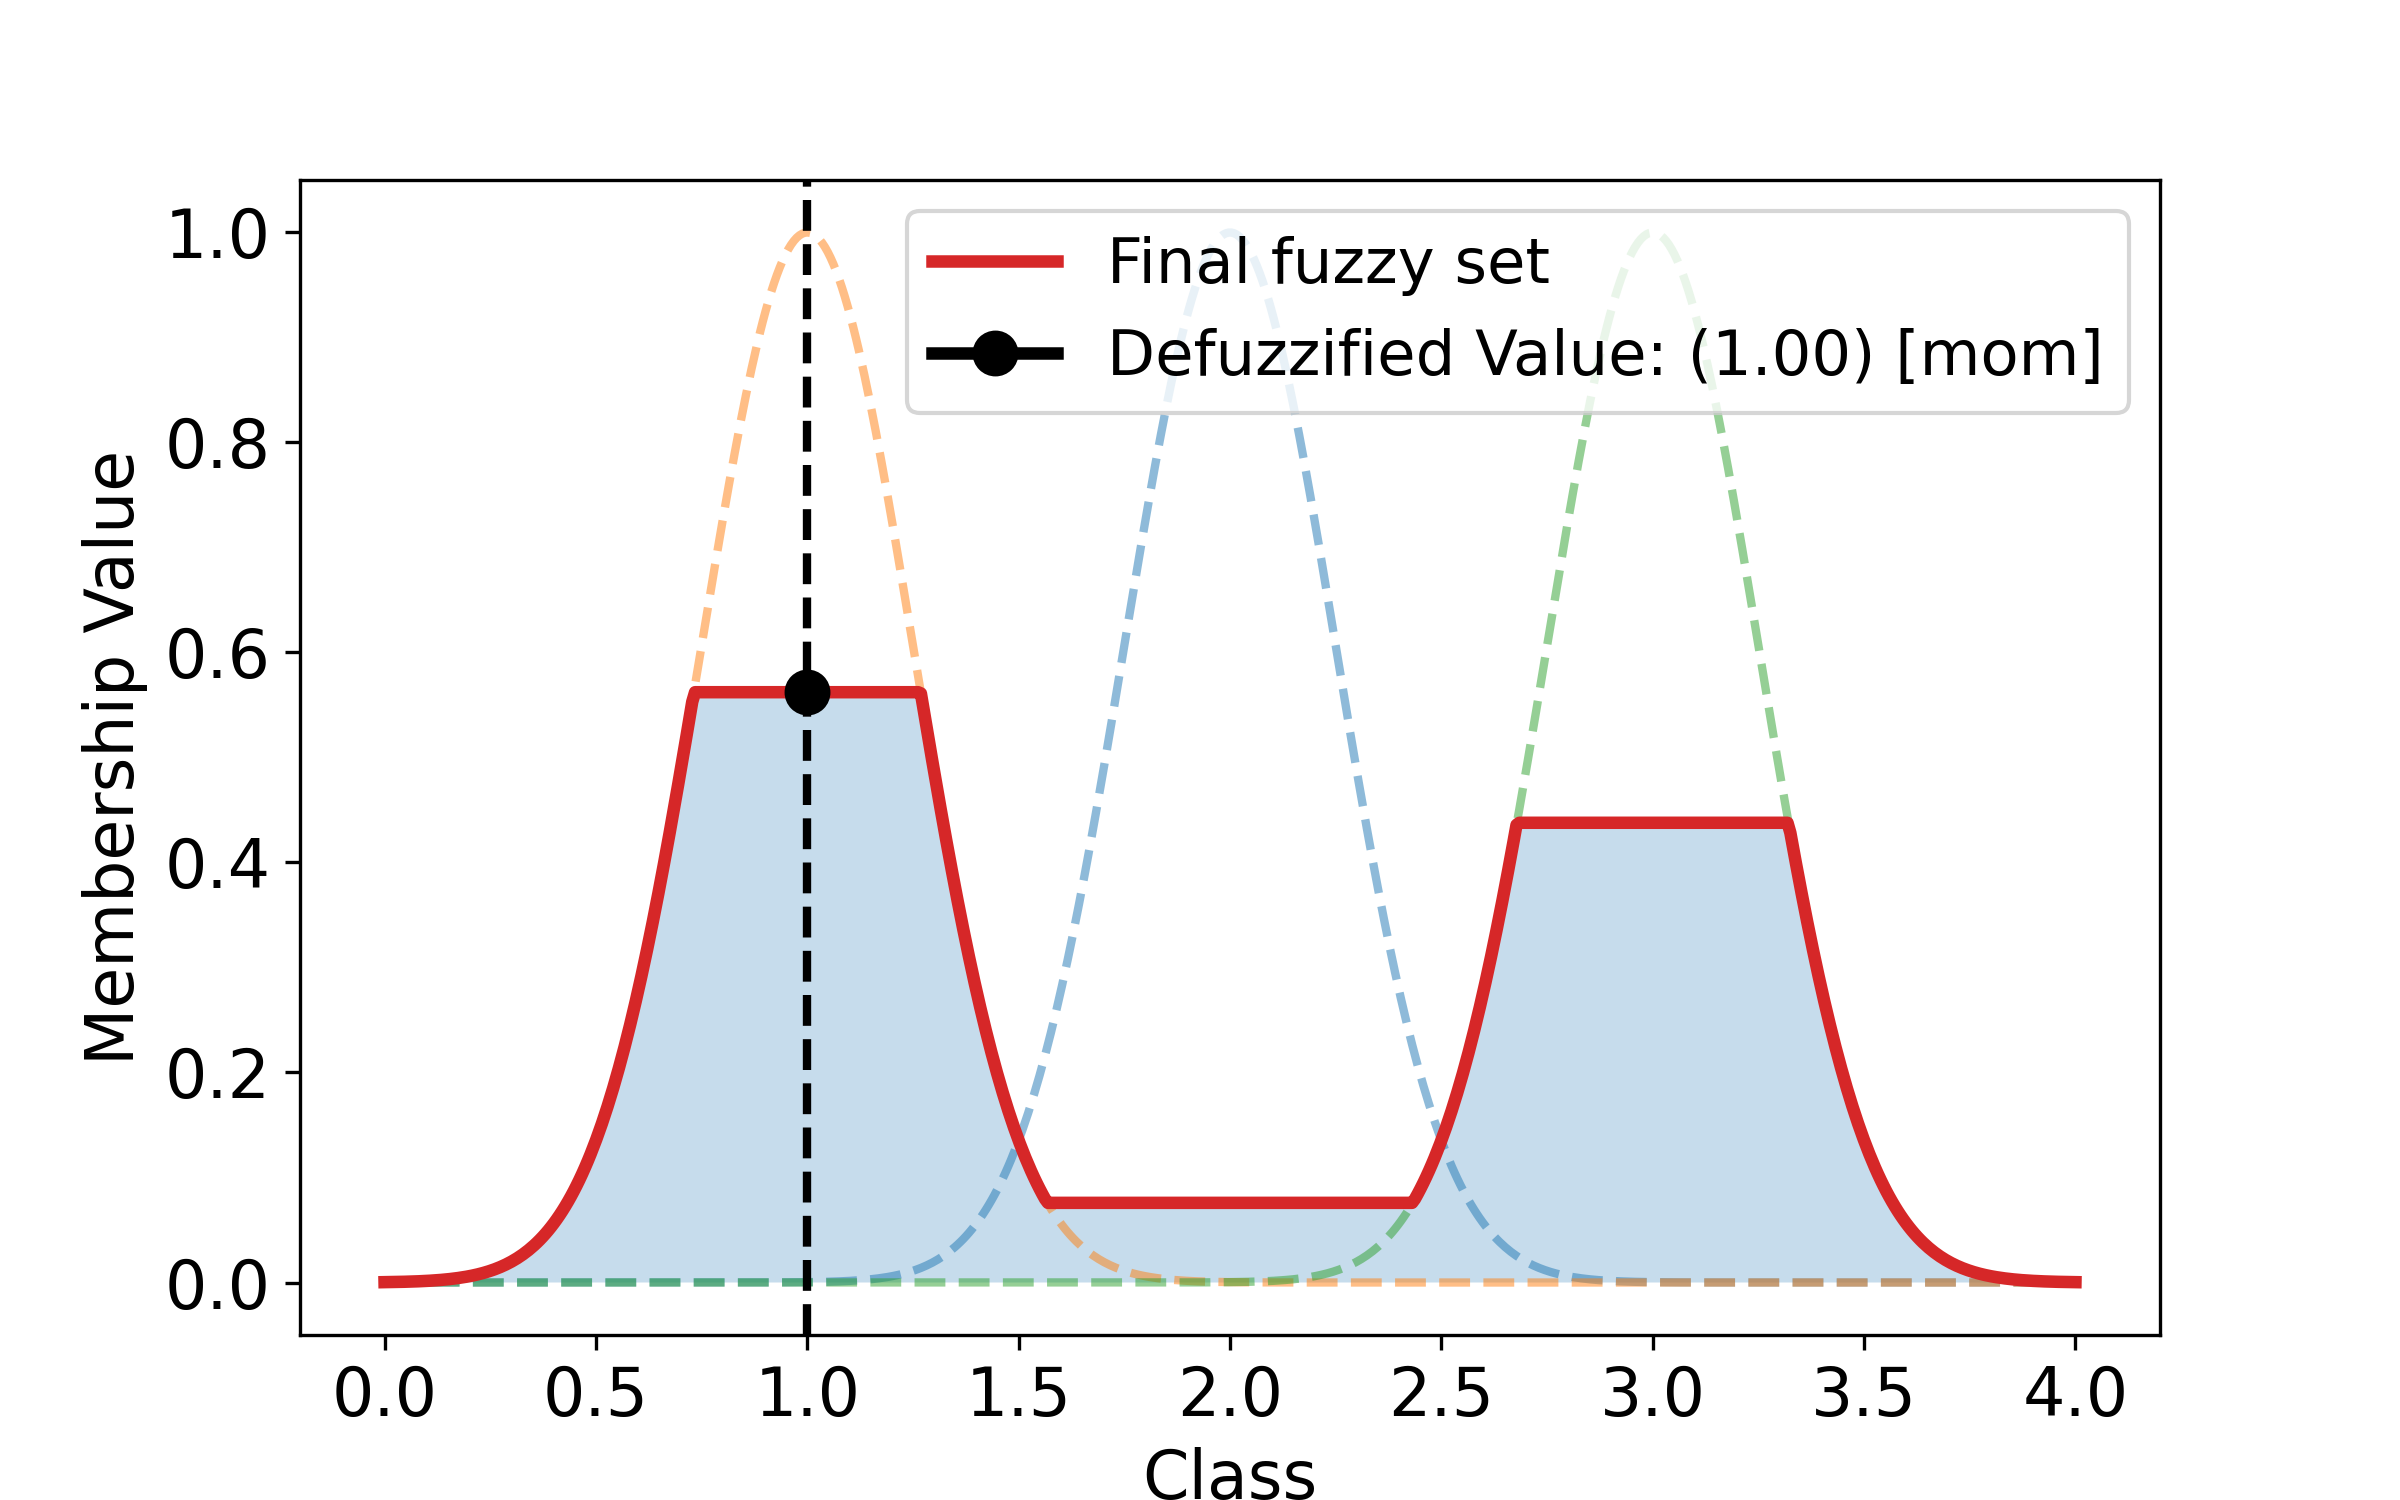
\includegraphics[width=\textwidth,trim={0 0 0 1cm},clip]{figures/ProofOfConcepts/fuzzy_set_for_data_mom.png}
        \caption[Resulting Fuzzy Set after applying the Rules on specific Data, MOM Method]{Defuzzification on the fuzzy obtained by applying the rules from \autoref{tab:fuzzyRulesExample} on the data point $(x=2.95, y=2.5)$. The \gls{mom} method correctly suggests the class value 1, as it is the class with the highest membership value.}
        \label{fig:fuzzySetForDataMOM}
    \end{subfigure}
    \caption{Comparison of COG and MOM defuzzification methods}
    \label{fig:fuzzySetComparison}
\end{figure}

As previously mentioned, we can recreate the process depicted in \autoref{fig:fuzzySystem} for every possible input data point to visualize the fuzzy systems' decision surface. Both resulting decision surfaces are shown in \autoref{fig:fuzzyDecisionSurfaceExampleCOG} and \autoref{fig:fuzzyDecisionSurfaceExampleMOM}, respectively. The decision surface using the \gls{cog} tries to smoothly interpolate between the different classes, which causes interpolation errors if there are other classes in between. The decision surface using the \gls{mom} method is valid and closely resembles the decision surface of the crisp decision tree in \autoref{fig:decisionBoundaryExample}.

\begin{figure}[H]
    \centering
    \begin{subfigure}[t]{0.48\textwidth}
        \centering
        \begin{tikzpicture}
            \node[anchor=south west,inner sep=0] (image) at (0,0) { 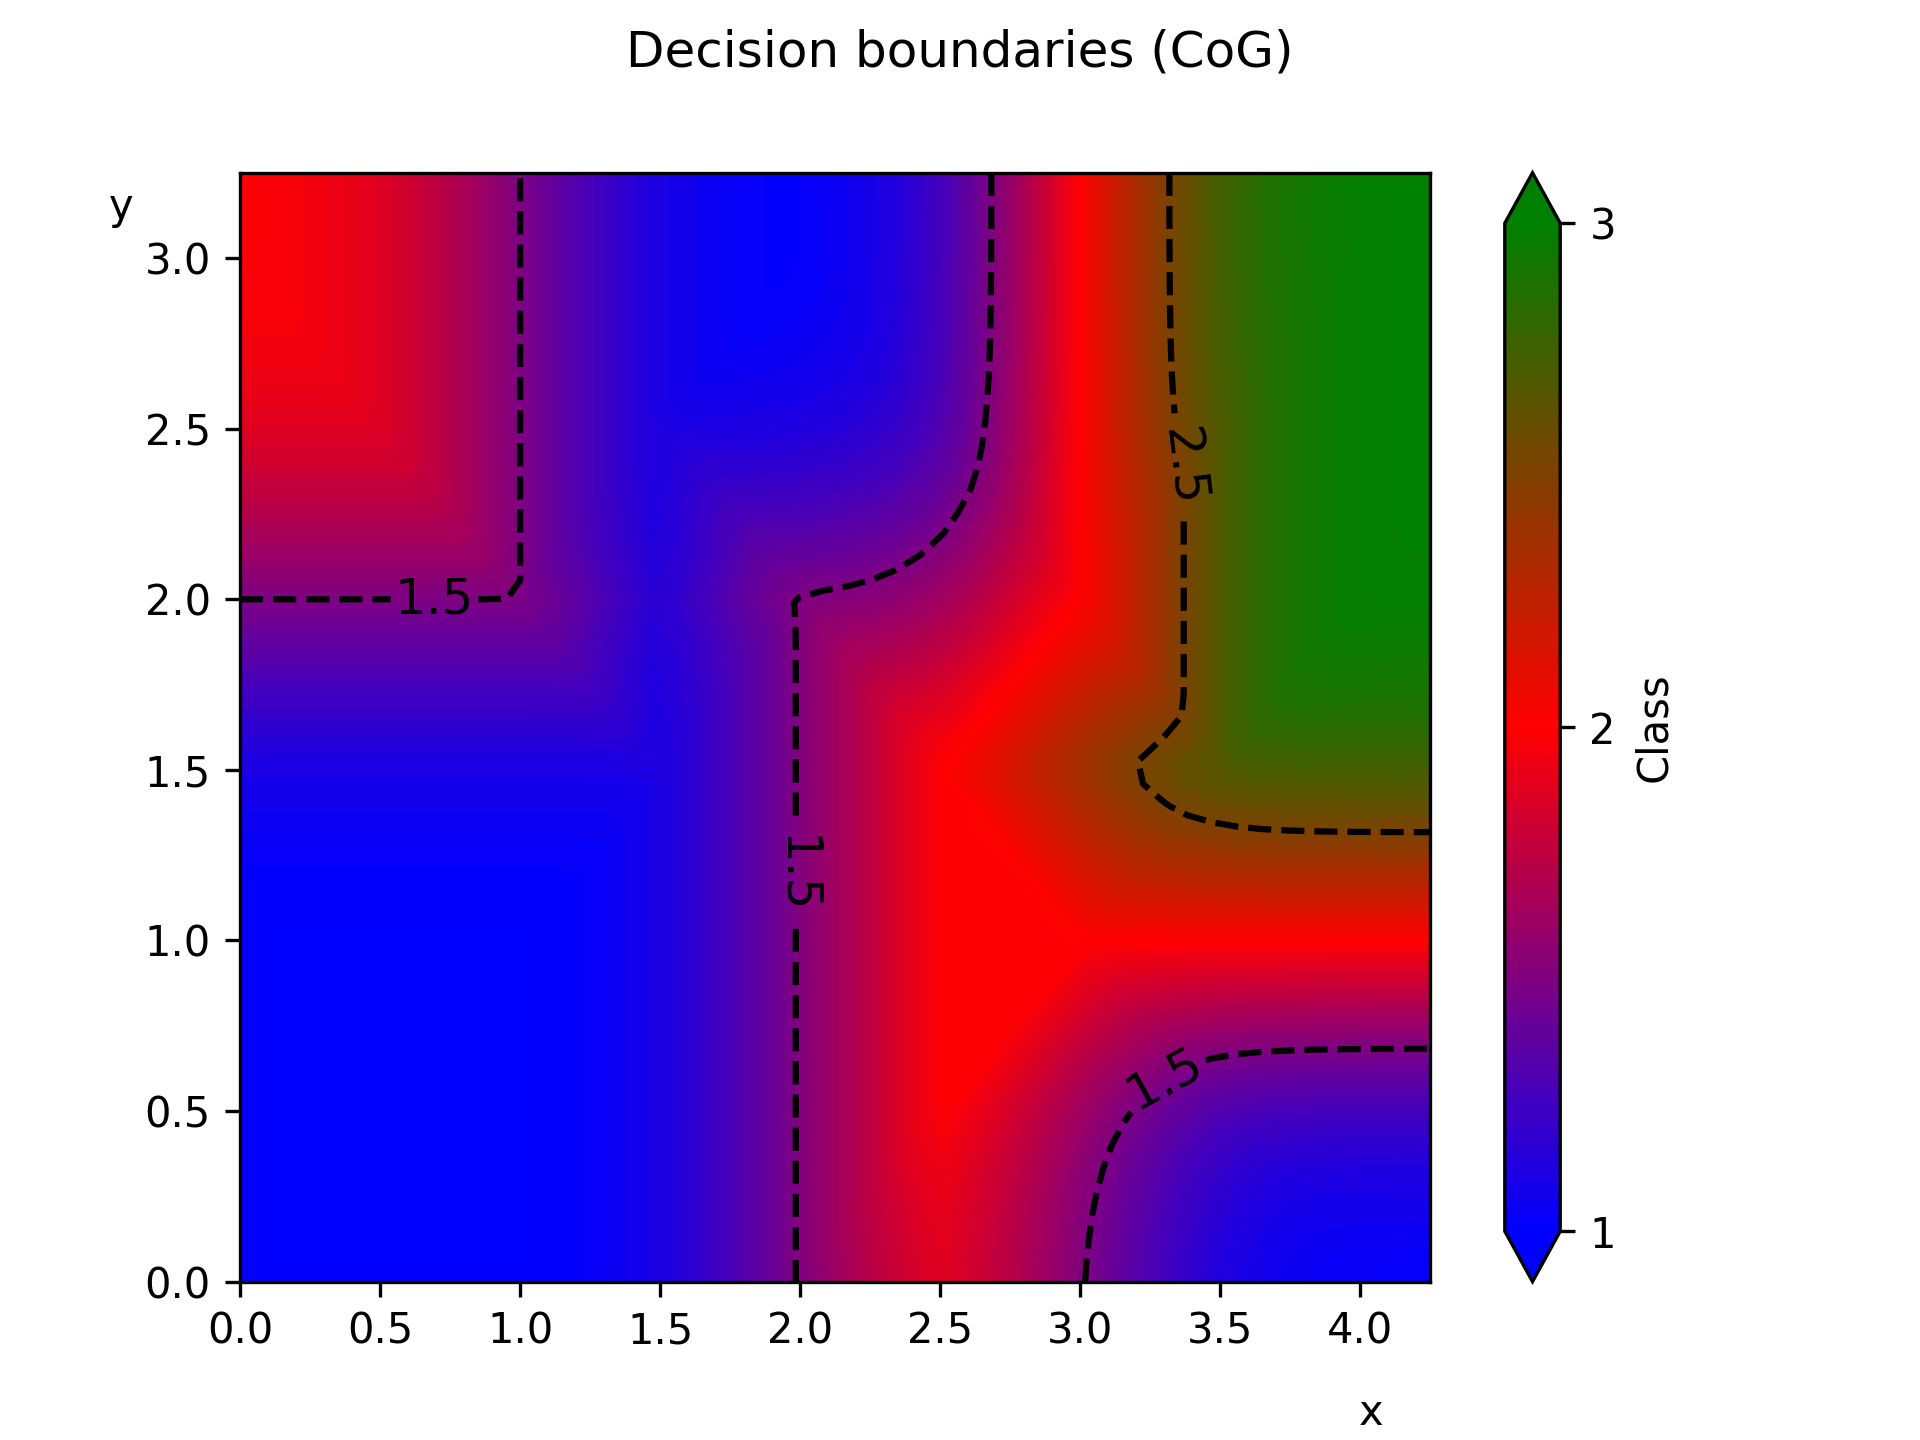
\includegraphics[width=\textwidth,trim={0 0 0 1.25cm},clip]{figures/ProofOfConcepts/fuzzy_system_cog.png}};
            \begin{scope}[x={(image.south east)},y={(image.north west)}]
                \draw[yellow, thin,rounded corners] (.55,.67) rectangle (.65,.95);
                \draw[yellow, thin,rounded corners] (.6,.32) rectangle (.74,.48);
                \node (A) at (.55,.56) [yellow, anchor=east] {\tiny{Interpolation Error}};

                \draw[yellow, arrow] (A) -- (.55,.67);
                \draw[yellow, arrow] (A) -- (.6,.48);
            \end{scope}
        \end{tikzpicture}
        \caption[Decision surface of the fuzzy rules using COG method]{Decision surface of the fuzzy-system using the \gls{cog} method. The highlighted areas show interpolation errors caused by the defuzzification.}
        \label{fig:fuzzyDecisionSurfaceExampleCOG}
    \end{subfigure}
    \hfill
    \begin{subfigure}[t]{0.48\textwidth}
        \centering
        \begin{tikzpicture}
            \node[anchor=south west,inner sep=0] (image) at (0,0) { 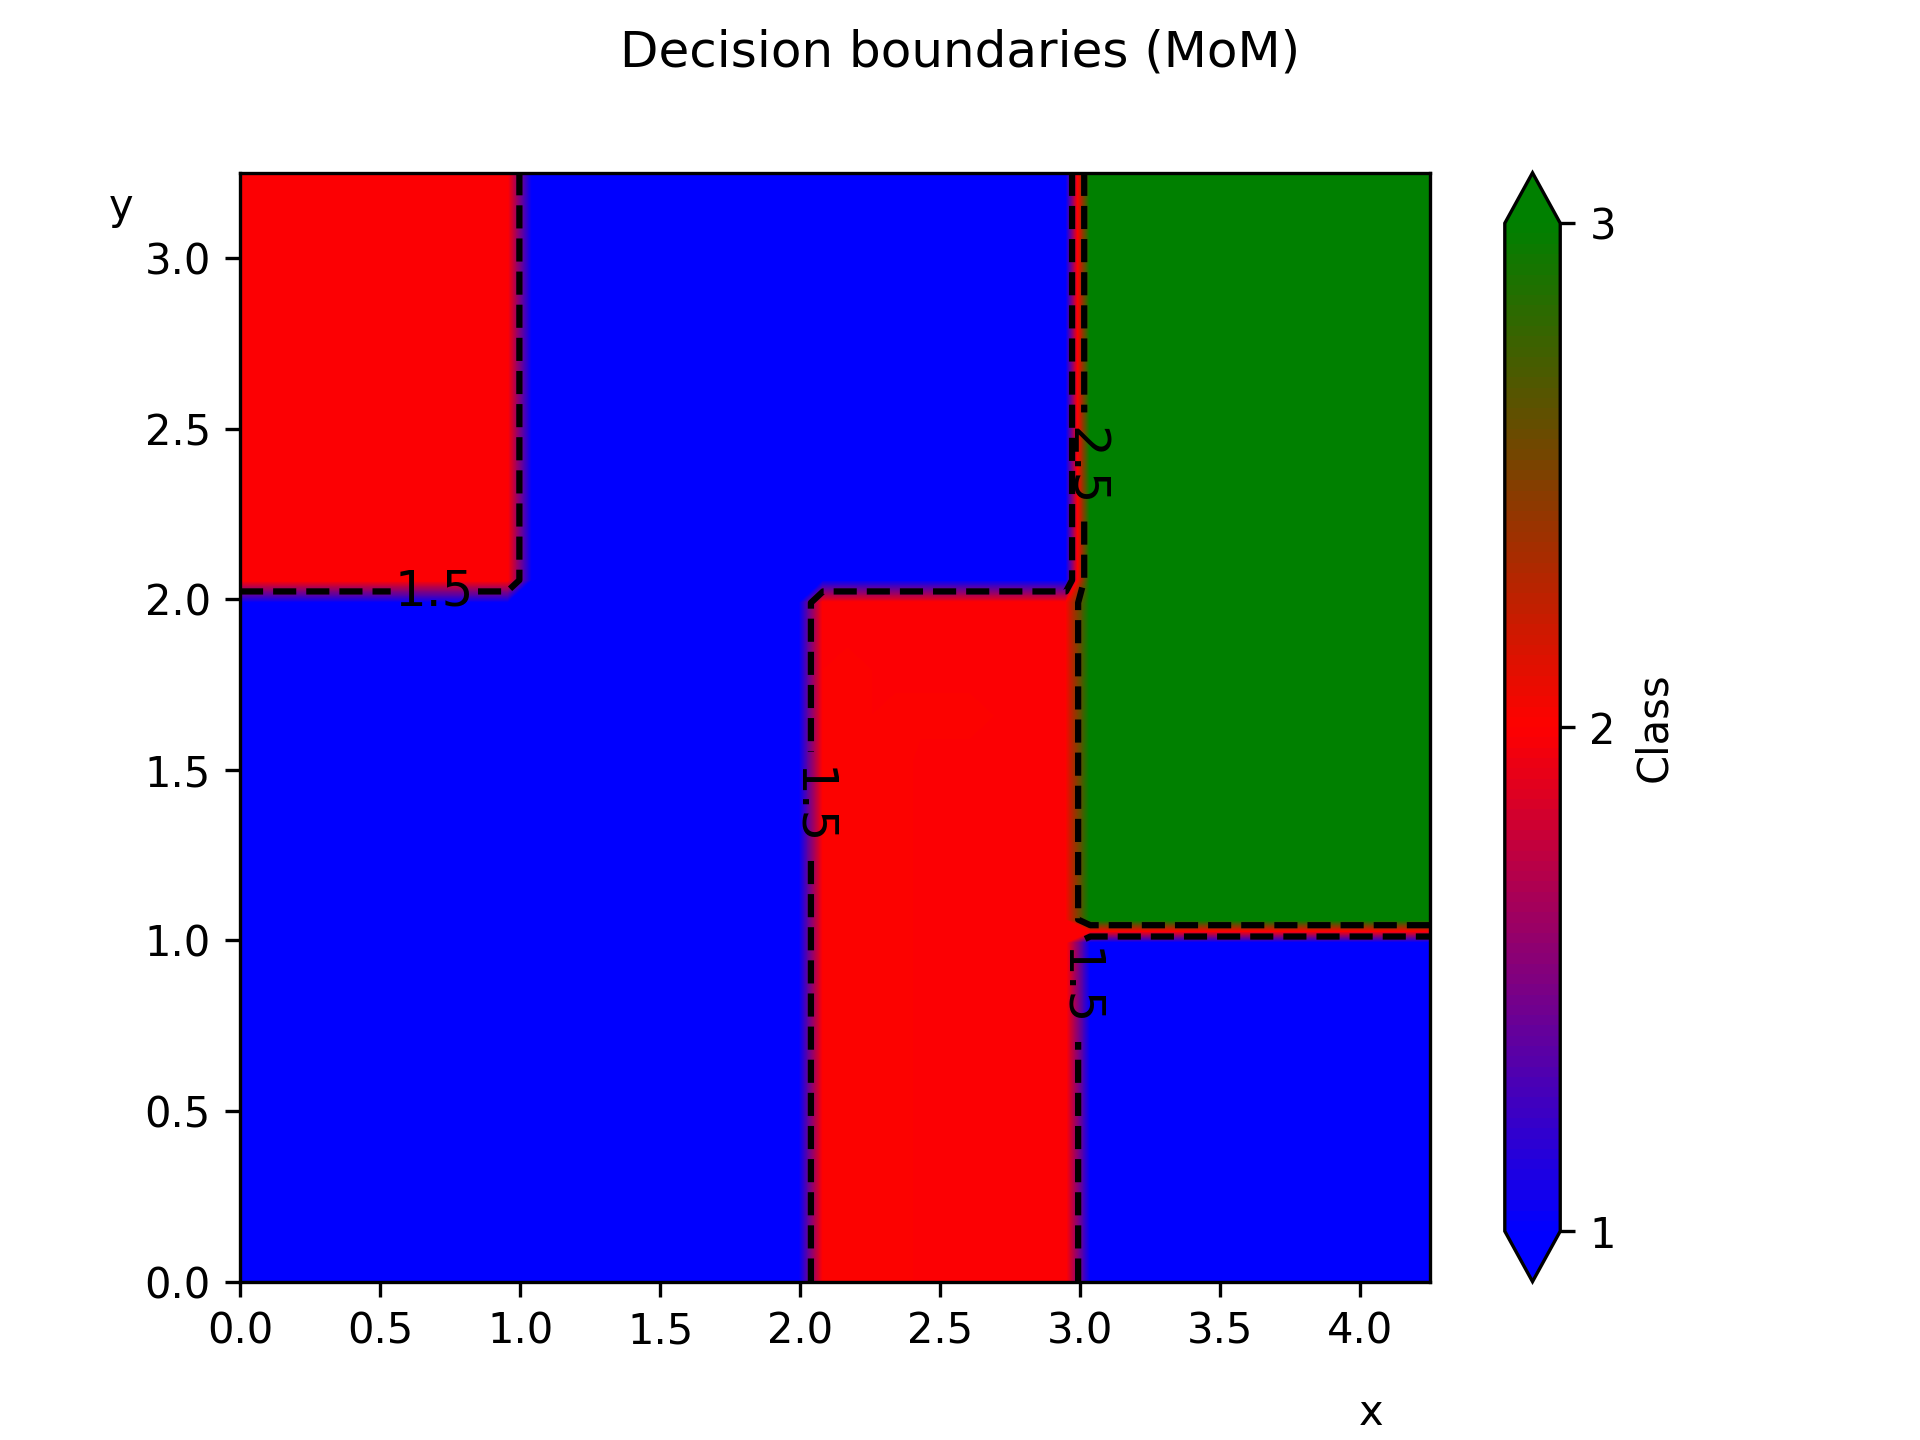
\includegraphics[width=\textwidth,trim={0 0 0 1.25cm},clip]{figures/ProofOfConcepts/fuzzy_system_mom.png}};
        \end{tikzpicture}
        \caption[Decision surface of the fuzzy rules using MOM method]{Decision surface of the fuzzy-system using the \gls{mom} method. There are no invalid regions in the decision surface.}
        \label{fig:fuzzyDecisionSurfaceExampleMOM}
    \end{subfigure}
    \caption{Comparison of COG and MOM defuzzification methods on decision surfaces}
    \label{fig:fuzzyDecisionSurfaceComparison}
\end{figure}


\section{Fuzzy Systems for \texttt{md\_flexible}}

This section will demonstrate how to generate fuzzy systems for \gls{mdflexible} simulations using the approach described in the previous section. The first section will describe the data collection process needed to train the classic decision trees, and the later sections will use the obtained data to generate two different styles of fuzzy systems for making predictions about the optimal configuration of the current simulation.

\subsection{Data Collection}

\subsubsection{Included Scenarios}

We chose to include the prominent example scenarios provided by \gls{mdflexible} such as \href{https://github.com/AutoPas/AutoPas/blob/c25dc770f173ff160630d7e58f59b38e277032a1/examples/md-flexible/input/fallingDrop.yaml}{\color{blue}\texttt{fallingDrop.yaml}}, \href{https://github.com/AutoPas/AutoPas/blob/c25dc770f173ff160630d7e58f59b38e277032a1/examples/md-flexible/input/explodingLiquid.yaml}{\color{blue} \texttt{explodingLiquid.yaml}} and \href{https://github.com/AutoPas/AutoPas/blob/c25dc770f173ff160630d7e58f59b38e277032a1/examples/md-flexible/input/SpinodalDecomposition.yaml}{\color{blue} \texttt{SpinodalDecomposition.yaml}} as the primary source of data. Additionally, we included some simulations of uniform cubes with different densities and particle counts to gather more data about the performance of the different configurations under lab-like conditions.

All simulations were run on the serial partition of the CoolMUC-2 cluster (see \ref*{CoolMucSpecs})  and were repeated twice to account for fluctuations in performance. Furthermore, every simulation was repeated with 1, 4, 12, 24, and 28 threads to additionally gather data on how parallelization affects the ideal configuration.

All the values were collected with the newly created \texttt{PAUSE\_SIMULATION\_DURING\_TUNING} CMake option enabled to ensure that the simulation state does not change during the tuning phases. This guarantees a fair comparison of the tested configurations, as all of them are evaluated under the exact same conditions. To gather the maximal amount of data, we used the \texttt{FullSeach} tuning strategy, which executes all possible configurations during the tuning phases.


\subsubsection{Collected Parameters}

The existing \texttt{TuningDataLogger} and the newly created \texttt{LiveInfoLogger} classes of the \gls{autopas} framework allow us to collect a wide variety of parameters during the simulation, such as the used configuration, information about the state of the simulation, and the measured timing data for each iteration of the simulation.

The complete shape of the collected data can be found in \autoref{des:tuningdatafields} and \autoref{des:liveinfodatafields}, respectively. We will however only make use of a subset of the available LiveInfo data, as we are only interested in \emph{relative} values that do not change when the simulation is scaled up or down and are therefore only primarily focus on: \texttt{avgParticlesPerCell}, \texttt{maxParticlesPerCell}, \texttt{homogeneity}, \texttt{maxDensity}, \texttt{particlesPerCellStdDev} and \texttt{threadCount}. This focus should help the fuzzy systems generalize better to unseen data, as they are less likely to overfit the training data.


\subsubsection{Limitations}

As the performance of machine learning models may degrade quickly when confronted with significantly different data than the data they were trained on, it is essential to collect a wide variety of scenarios to cover as many possible use cases as possible. As we only included a limited number of scenarios, we have to keep in mind that the generated fuzzy systems will only be able to make confident predictions about scenarios similar to the included ones, and we should not expect them to generalize well to unseen data.
To guarantee a fair evaluation of this tuning approach, we will only focus on slight variations of the included scenarios in the following evaluation section.

\subsection{Data Preprocessing}

In order to make predictions about the performance of different configurations, we first need to define an appropriate metric to compare them. As we \emph{froze} the simulation during the tuning process with the \texttt{PAUSE\_SIMULATION\_DURING\_TUNING} option, we can safely use the runtimes of the different configurations to compare them. Those runtimes are, however, absolute values and may differ significantly between tuning phases as the underlying simulation changes. To compare runtimes between different tuning phases, we introduce the concept of \emph{relative speed}, which measures how well a configuration performs compared to the best configuration in the same tuning phase, and augment the collected timing data with this metric. The relative speed is calculated as


\begin{equation}
    {\text{relative speed}^{(i)}_{\text{config}}}= \frac{t_{\text{best}}^{(i)}}{t_{\text{config}}^{(i)}}
\end{equation}

Where $t_{\text{best}}^{(i)}$ is the runtime of the best configuration during the $i$-th tuning phase and $t_{\text{config}}^{(i)}$ is the runtime of the configuration we are interested in.

This value will range from 0 (being infinitely worse than the best configuration) to 1 (being equally good as the best configuration) for each configuration. Additionally, we chose to combine the fields \texttt{Container} and \texttt{DataLayout} of the configuration into a single field \texttt{ContainerDataLayout} as they are closely related, and the performance of one is heavily dependent on the other.

We can now create the augmented dataset shown in \autoref{tab:trainingData}, which will be used in the following sections to train the decision trees and generate the fuzzy systems.


\definecolor{LightCyan}{rgb}{0.88,1,1}
\newcolumntype{g}{>{\columncolor{LightCyan}}c}
\begin{table}[H]
    \centering
    \tiny
    \def\arraystretch{2.5}
    \begin{tabular}{|c|c|c|c|c|c|c|c|c| g|}
        \cline{1-9}
        \multicolumn{3}{|c|}{ \textbf{ParticlesPerCell}} & \multicolumn{3}{c|}{\textbf{Miscellaneous}} & \multicolumn{3}{c|}{\textbf{Configuration}}                                                                                                                           \\
        \hline
        \textbf{avg}                                     & \textbf{max}                                & \textbf{stddev}                             & \tabularCenterstack{c}{\textbf{homo-}                                                                                   \\ \textbf{genity}} & \tabularCenterstack{c}{\textbf{max-} \\ \textbf{density}} & \textbf{threads} & \tabularCenterstack{c}{\textbf{Container} \\ \textbf{DataLayout}}& \textbf{Traversal} & \textbf{Newton3} & \textbf{Relative speed} \\
        \hline
        0.905                                            & 23                                          & 0.0129                                      & 0.0354                                & 0.531  & 1      & LinkedCells\_AoS      & lc\_sliced      & enabled  & 0.450641 \\
        2.201                                            & 13                                          & 0.0144                                      & 0.0861                                & 0.627  & 24     & VerletListsCells\_AoS & vlc\_sliced     & disabled & 0.594117 \\
        0.905                                            & 18                                          & 0.0136                                      & 0.0431                                & 0.319  & 4      & LinkedCells\_AoS      & lc\_sliced\_c02 & enabled  & 0.454632 \\
        \vdots                                           & \vdots                                      & \vdots                                      & \vdots                                & \vdots & \vdots & \vdots                & \vdots          & \vdots   & \vdots   \\
        \hline
    \end{tabular}
    \caption[Augmented dataset used for creating the fuzzy systems]{Augmented dataset used for creating the fuzzy systems. The dataset contains the average, maximum, and standard deviation of the particles per cell, the homogeneity, density, and thread count of the simulation, as well as the configuration options and the relative speed of the configuration compared to the best configuration in the same tuning phase.}
    \label{tab:trainingData}
\end{table}


As described previously, we will create two different kinds of knowledge bases using this dataset. The first attempt is called \emph{Component Tuning Approach} and tries to independently predict the best options for each tunable parameter. The second attempt is the \emph{Suitability Tuning Approach}, which tries to predict the $relative speed$ values for all possible configurations and then selects the configurations expected to perform best. Both approaches will be described in the following sections.

\subsection{Component Tuning Approach}

This approach makes use of three different \texttt{FuzzySystems}, one for each of the tunable parameters of the simulation (\texttt{ContainerDataLayout}, \texttt{Traversal}, and \texttt{Newton3}). All those systems should independently predict the best configuration for their respective parameter based on the current LiveInfoData. \autoref{fig:fuzzySystemComponent} shows the structure of this approach.

As we only want to create a fuzzy system predicting appropriate configurations, we naively remove all configurations performing worse than a certain suitability threshold (we chose 70\%) as depicted in \autoref{fig:relativeSpeed}. The remaining configurations, which are known to perform well, are then used to create the fuzzy systems.


\begin{figure}[H]
    \centering
    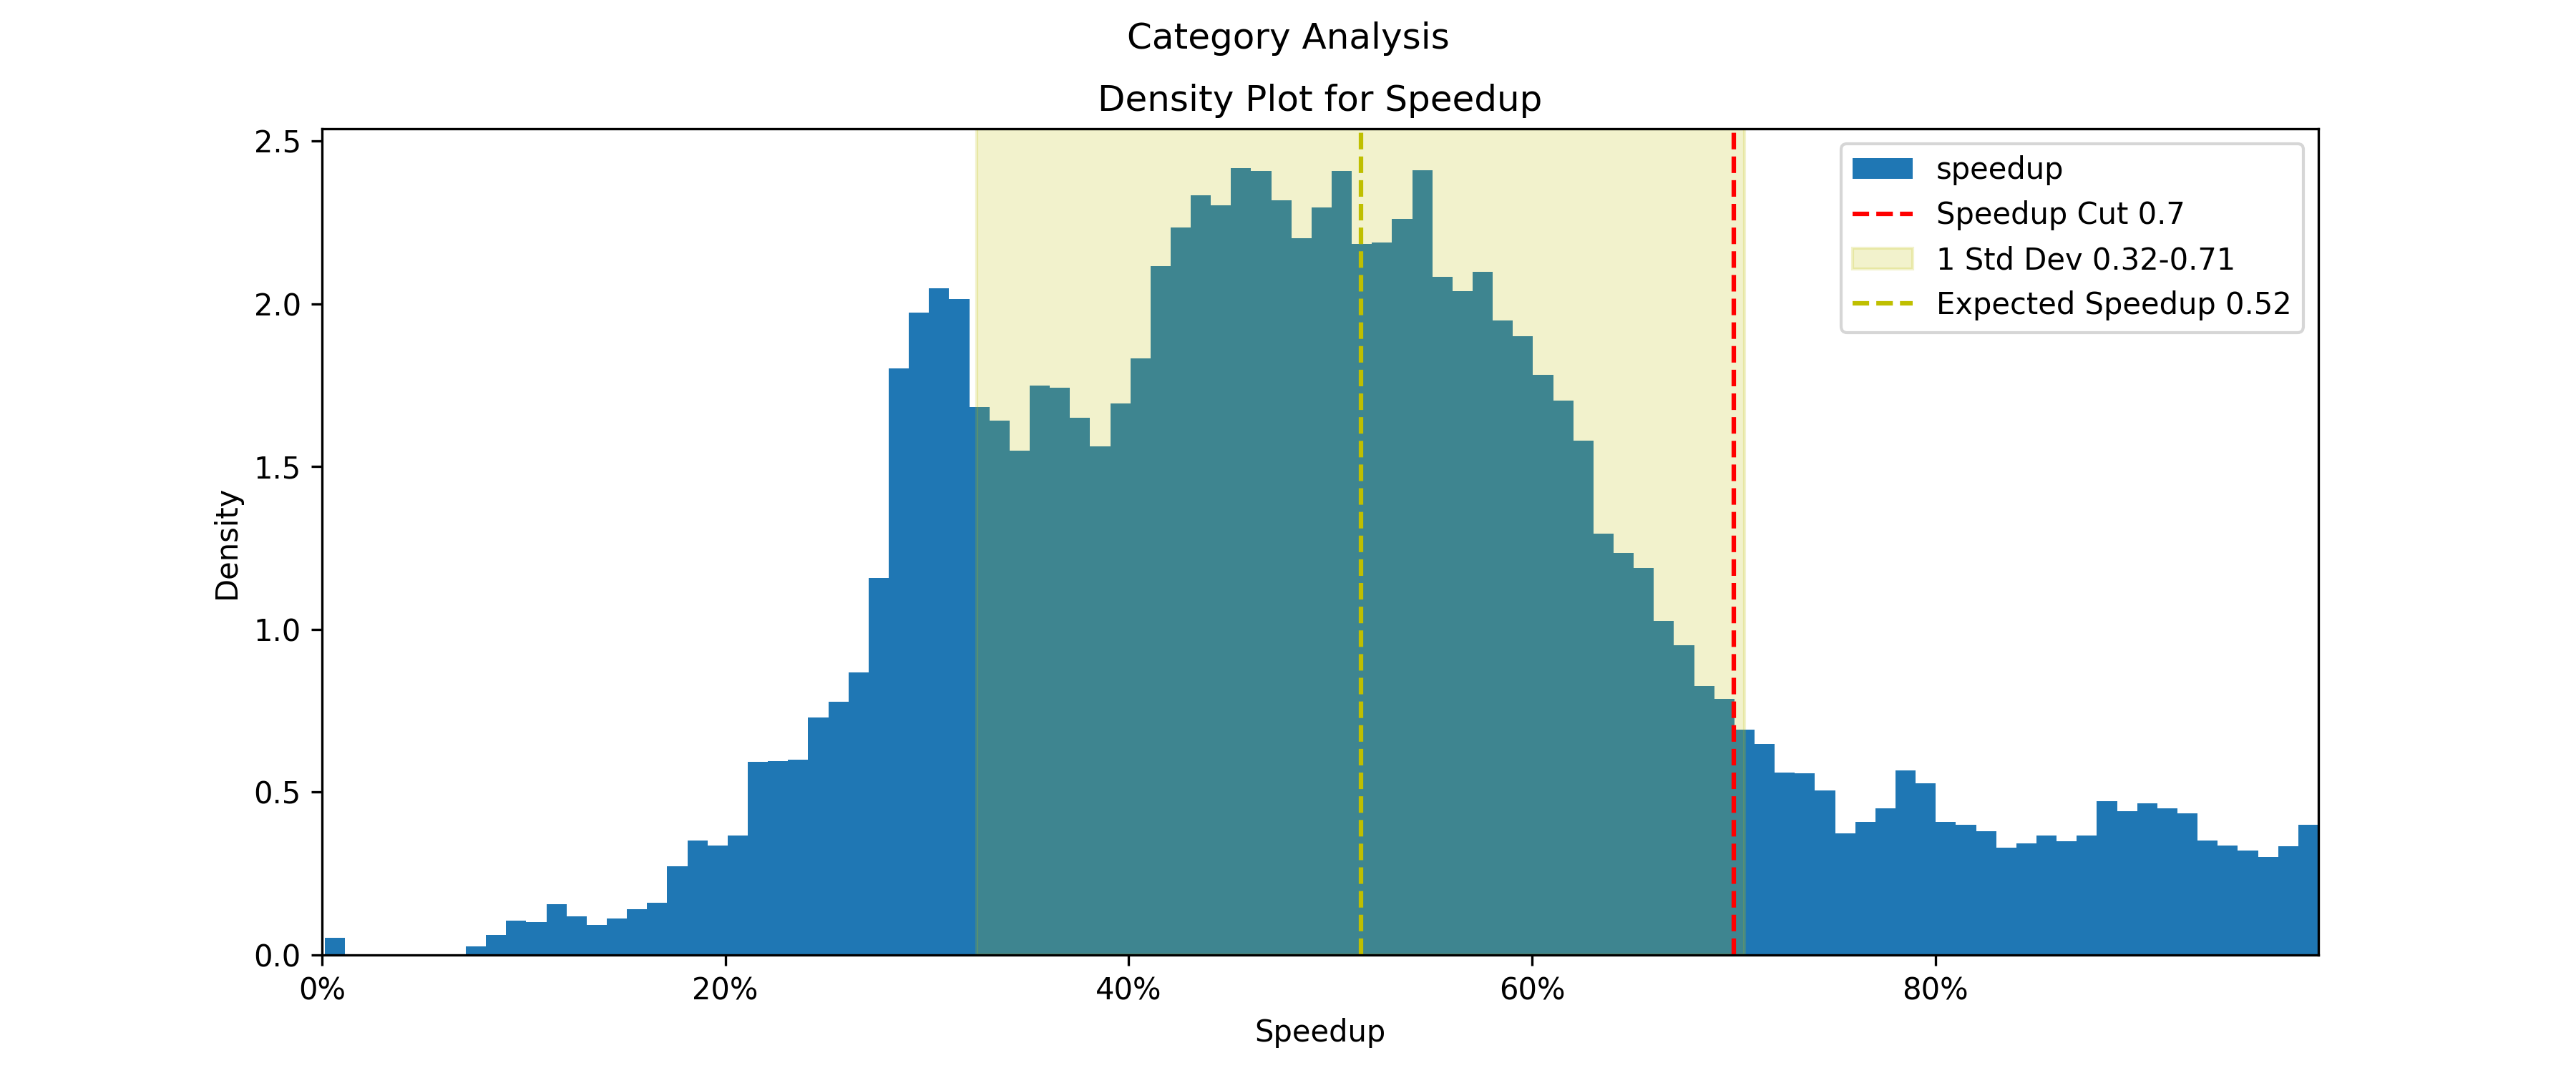
\includegraphics[width=\columnwidth,trim={1cm 0 2cm 1.5cm},clip]{figures/DataAnalytics/speedup.png}
    \caption[Relative speed distribution of the collected data]{Relative speed distribution of the collected data. The suitability threshold is set to 70\%, thus removing all configurations performing worse than this threshold. From the plot, we can also see that the average configuration performs just 52\% as well as the best configuration, with some configurations also performing ten times worse than the best in certain tuning phases.}
    \label{fig:relativeSpeed}
\end{figure}

Afterward, we group all configurations evaluated in the same tuning phase and aggregate all the present values of tunable parameters into a single term. As we \emph{froze} the simulation during the tuning phase, the LiveInfoData will be equal for such configurations, and the aggregated terms will therefore represent all \emph{good} values for the parameters in this simulation state (as they occur in configurations with $\geq 70\%$ suitability). The aggregated training data is shown in \autoref{tab:trainingDataComponent} and is used to fit three decision trees, which are then converted into fuzzy systems using the method described in the previous section. A few of the extracted fuzzy rules are shown in \autoref{tab:fuzzyRulesComponent}. The linguistic variables are omitted for brevity.

\begin{table}[H]
    \centering
    \tiny
    \def\arraystretch{2.5}
    \begin{tabular}{|c|c|c|c|c|c|c|c|c|}
        \cline{1-9}
        \multicolumn{3}{|c|}{ \textbf{ParticlesPerCell}} & \multicolumn{3}{c|}{\textbf{Miscellaneous}} & \multicolumn{3}{c|}{\textbf{Aggregated Configuration Terms}}                                                                                                                               \\
        \hline
        \textbf{avg}                                     & \textbf{max}                                & \textbf{stddev}                                              & \tabularCenterstack{c}{\textbf{homo-}                                                                                       \\ \textbf{genity}} & \tabularCenterstack{c}{\textbf{max-} \\ \textbf{density}} & \textbf{threads} & \tabularCenterstack{c}{\textbf{Container} \\ \textbf{DataLayout}}& \textbf{Traversal} & \textbf{Newton3}  \\
        \hline
        0.906                                            & 15                                          & 0.015                                                        & 0.055                                 & 0.297  & 4      & \tabularCenterstack{c}{"LinkedCells\_SoA,                         \\ VerletClusterLists\_SoA, \\ VerletListsCells\_AoS"} & \tabularCenterstack{c}{"lc\_sliced, \\ lc\_sliced\_balanced, \\ lc\_sliced\_c02"} & "enabled"   \\
        \hline
        0.945                                            & 25                                          & 0.041                                                        & 0.084                                 & 0.673  & 24     & \tabularCenterstack{c}{"LinkedCells\_SoA,                         \\ VerletClusterLists\_SoA, \\ VerletListsCells\_AoS"} & \tabularCenterstack{c}{"lc\_c04, \\ lc\_c08, \\ lc\_sliced, \\ lc\_sliced\_balanced"} & \tabularCenterstack{c}{"disabled, \\ enabled"}  \\
        \hline
        0.906                                            & 20                                          & 0.014                                                        & 0.041                                 & 0.336  & 24     & \tabularCenterstack{c}{VerletClusterLists\_SoA,                   \\ VerletListsCells\_AoS} & \tabularCenterstack{c}{"vcl\_c06, \\ vlc\_c01, \\ vlc\_c18"} & \tabularCenterstack{c}{"disabled, \\ enabled"} \\
        \hline
        \vdots                                           & \vdots                                      & \vdots                                                       & \vdots                                & \vdots & \vdots & \vdots                                          & \vdots & \vdots \\
        \hline
    \end{tabular}
    \caption[Aggregated training data for the Component Tuning Approach]{Aggregated training data for the Component Tuning Approach. Each row represents a different tuning phase. The numerical values stem from the LiveInfoData during that tuning phase, and the aggregated configuration terms represent the configuration options that are known to perform well under the given conditions.}
    \label{tab:trainingDataComponent}
\end{table}


\begin{table}[H]
    \footnotesize
    \centering
    \addtolength{\leftskip} {-3cm} % increase (absolute) value if needed
    \addtolength{\rightskip}{-3cm}

    \begin{tabular}{|c|c|c|c|g|}
        \multicolumn{4}{c}{\large{\textbf{Antecedent}}} & \multicolumn{1}{c}{\large{\textbf{Consequent}    }}                                                                                                                                    \\
        \hline
        \textbf{avgParticlesPC}                         & \textbf{homogeneity}                                & \textbf{particlesPCStdDev}                        & \textbf{threadCount}      & \textbf{ContainerDataLayout}                     \\

        \hline
        \texttt{lower than 3.45}                        & \texttt{lower than 0.05}                            &                                                   & \texttt{lower than 18.0}  & \tabularCenterstack{c}{"VerletClusterLists\_SoA, \\
        VerletListsCells\_AoS"}                                                                                                                                                                                                                  \\
        \hline
        \texttt{lower than 3.45}                        & \texttt{higher than 0.05}                           & \texttt{lower than 0.024}                         & \texttt{higher than 18.0} & \tabularCenterstack{c}{"LinkedCells\_SoA,        \\ VerletClusterLists\_SoA,\\ VerletListsCells\_AoS"}  \\
        \hline
        \vdots                                          & \vdots                                              & \vdots                                            & \vdots                    & \vdots                                           \\
        \hline

        \multicolumn{5}{c}{ }                                                                                                                                                                                                                    \\


        \multicolumn{4}{c}{\large{\textbf{Antecedent}}} & \multicolumn{1}{c}{\large{\textbf{Consequent}    }}                                                                                                                                    \\

        \hline
        \textbf{avgParticlesPC}                         & \textbf{homogeneity}                                & \textbf{particlesPCStdDev}                        & \textbf{threadCount}      & \textbf{Traversal}                               \\

        \hline

        \texttt{lower than 1.553}                       & \texttt{higher than 0.047}                          & \texttt{lower than 0.023	}                         & \texttt{higher than 2.5}  & \tabularCenterstack{c}{"lc\_sliced,              \\ vlc\_c18,\\ lc\_sliced\_c02"}
        \\
        \hline

                                                        & \texttt{lower than 0.037}                           & \texttt{lower than 0.023	}                         & \texttt{lower than 26.0}  & \tabularCenterstack{c}{"vcl\_c06,                \\ vlc\_c18,\\ vlc\_sliced\_c02"}                                                          \\


        \hline
        \vdots                                          & \vdots                                              & \vdots                                            & \vdots                    & \vdots                                           \\
        \hline


        \multicolumn{5}{c}{ }                                                                                                                                                                                                                    \\


        \multicolumn{4}{c}{\large{\textbf{Antecedent}}} & \multicolumn{1}{c}{\large{\textbf{Consequent}    }}                                                                                                                                    \\

        \hline
        \textbf{avgParticlesPC}                         & \textbf{homogeneity}                                & \textbf{particlesPCStdDev}                        & \textbf{threadCount}      & \textbf{Newton 3}                                \\

        \hline

                                                        &                                                     & \texttt{higher than 0.03}                         & \texttt{higher than 18.0} & \tabularCenterstack{c}{"disabled,                \\enabled"}
        \\
        \hline

                                                        &                                                     & \tabularCenterstack{c}{\texttt{higher than 0.023}                                                                                \\ $\land$ \texttt{lower than 0.037	}} &  \tabularCenterstack{c}{\texttt{lower than 18.0}\\ $\land$ \texttt{higher than 8.0	}} & \tabularCenterstack{c}{"enabled"}                \\


        \hline
        \vdots                                          & \vdots                                              & \vdots                                            & \vdots                    & \vdots                                           \\
        \hline
    \end{tabular}

    \caption[Extracted fuzzy rules from the decision trees for the Component Tuning Approach]{Extracted fuzzy rules from the decision trees for the Component Tuning Approach. The rules are grouped by the tunable parameter they predict. The first row is read as:
        \footnotesize{$\text{IF} \;  (\text{avgParticlesPC} = \text{"lower than 3.454"})  \land   (\text{homogeneity} = \text{"lower than 0.05"})   \land (\text{threadCount} = \text{"lower than 18.0"}) \; \text{THEN} \; (\text{ContainerDataLayout} = \text{"VerletClusterLists\_SoA, VerletListsCells\_AoS"})$}}
    \label{tab:fuzzyRulesComponent}
\end{table}

\newpage

As described previously, we use \texttt{gaussian} membership functions for each linguistic term of the consequent linguistic variables. The placement of the values is irrelevant as we will use the \gls{mom} defuzzification method. \autoref{fig:homogenityLinguisticVariable} and \autoref{fig:newton3LinguisticVariable_component} show the resulting linguistic variables for the homogeneity linguistic variable (an input variable) and the Newton3 linguistic variable we want to predict. The visualization of the other variables follows a similar pattern but is more complex due to the higher number of terms and are therefore not shown here.



\begin{multicols}{2}
    \begin{figure}[H]
        \centering
        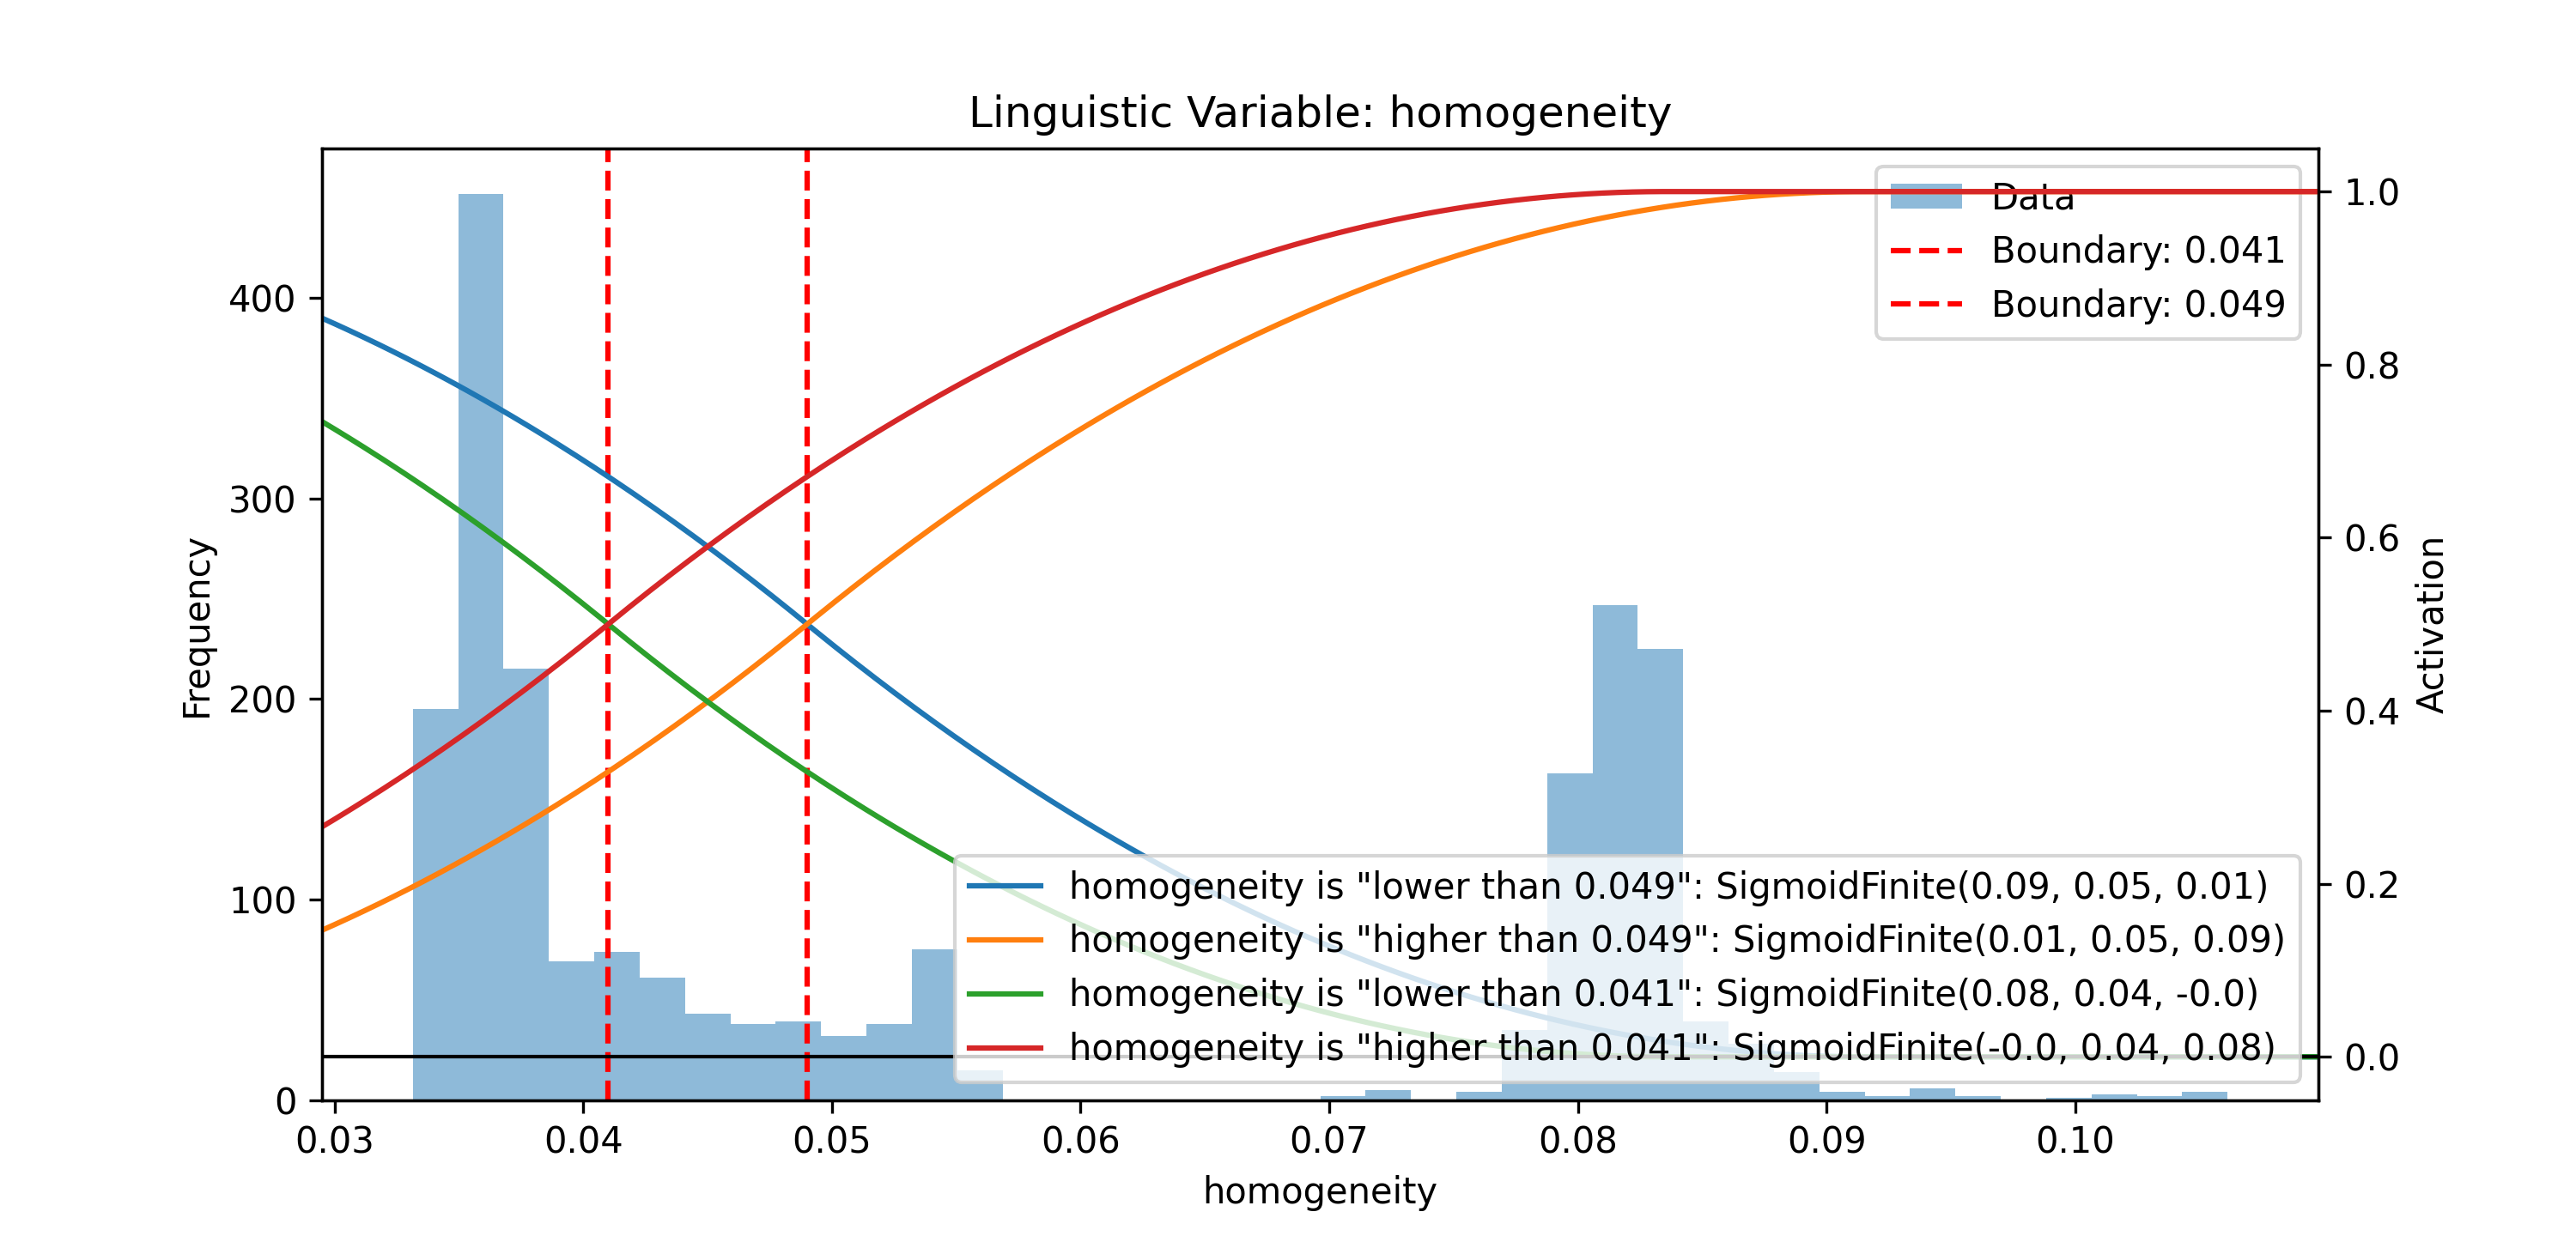
\includegraphics[width=\columnwidth,trim={1cm 0 1cm 1.35cm},clip]{figures/DataAnalytics/homogenity_linguistic_variable.png}

        \caption[Linguistic variable for the homogeneity attribute]{
            This figure shows the linguistic variable for the homogeneity attribute. We see the different fuzzy sets created from the decision trees. The background shows the histogram of all homogeneity values present in the dataset.
        }
        \label{fig:homogenityLinguisticVariable}
    \end{figure}

    \columnbreak

    \begin{figure}[H]
        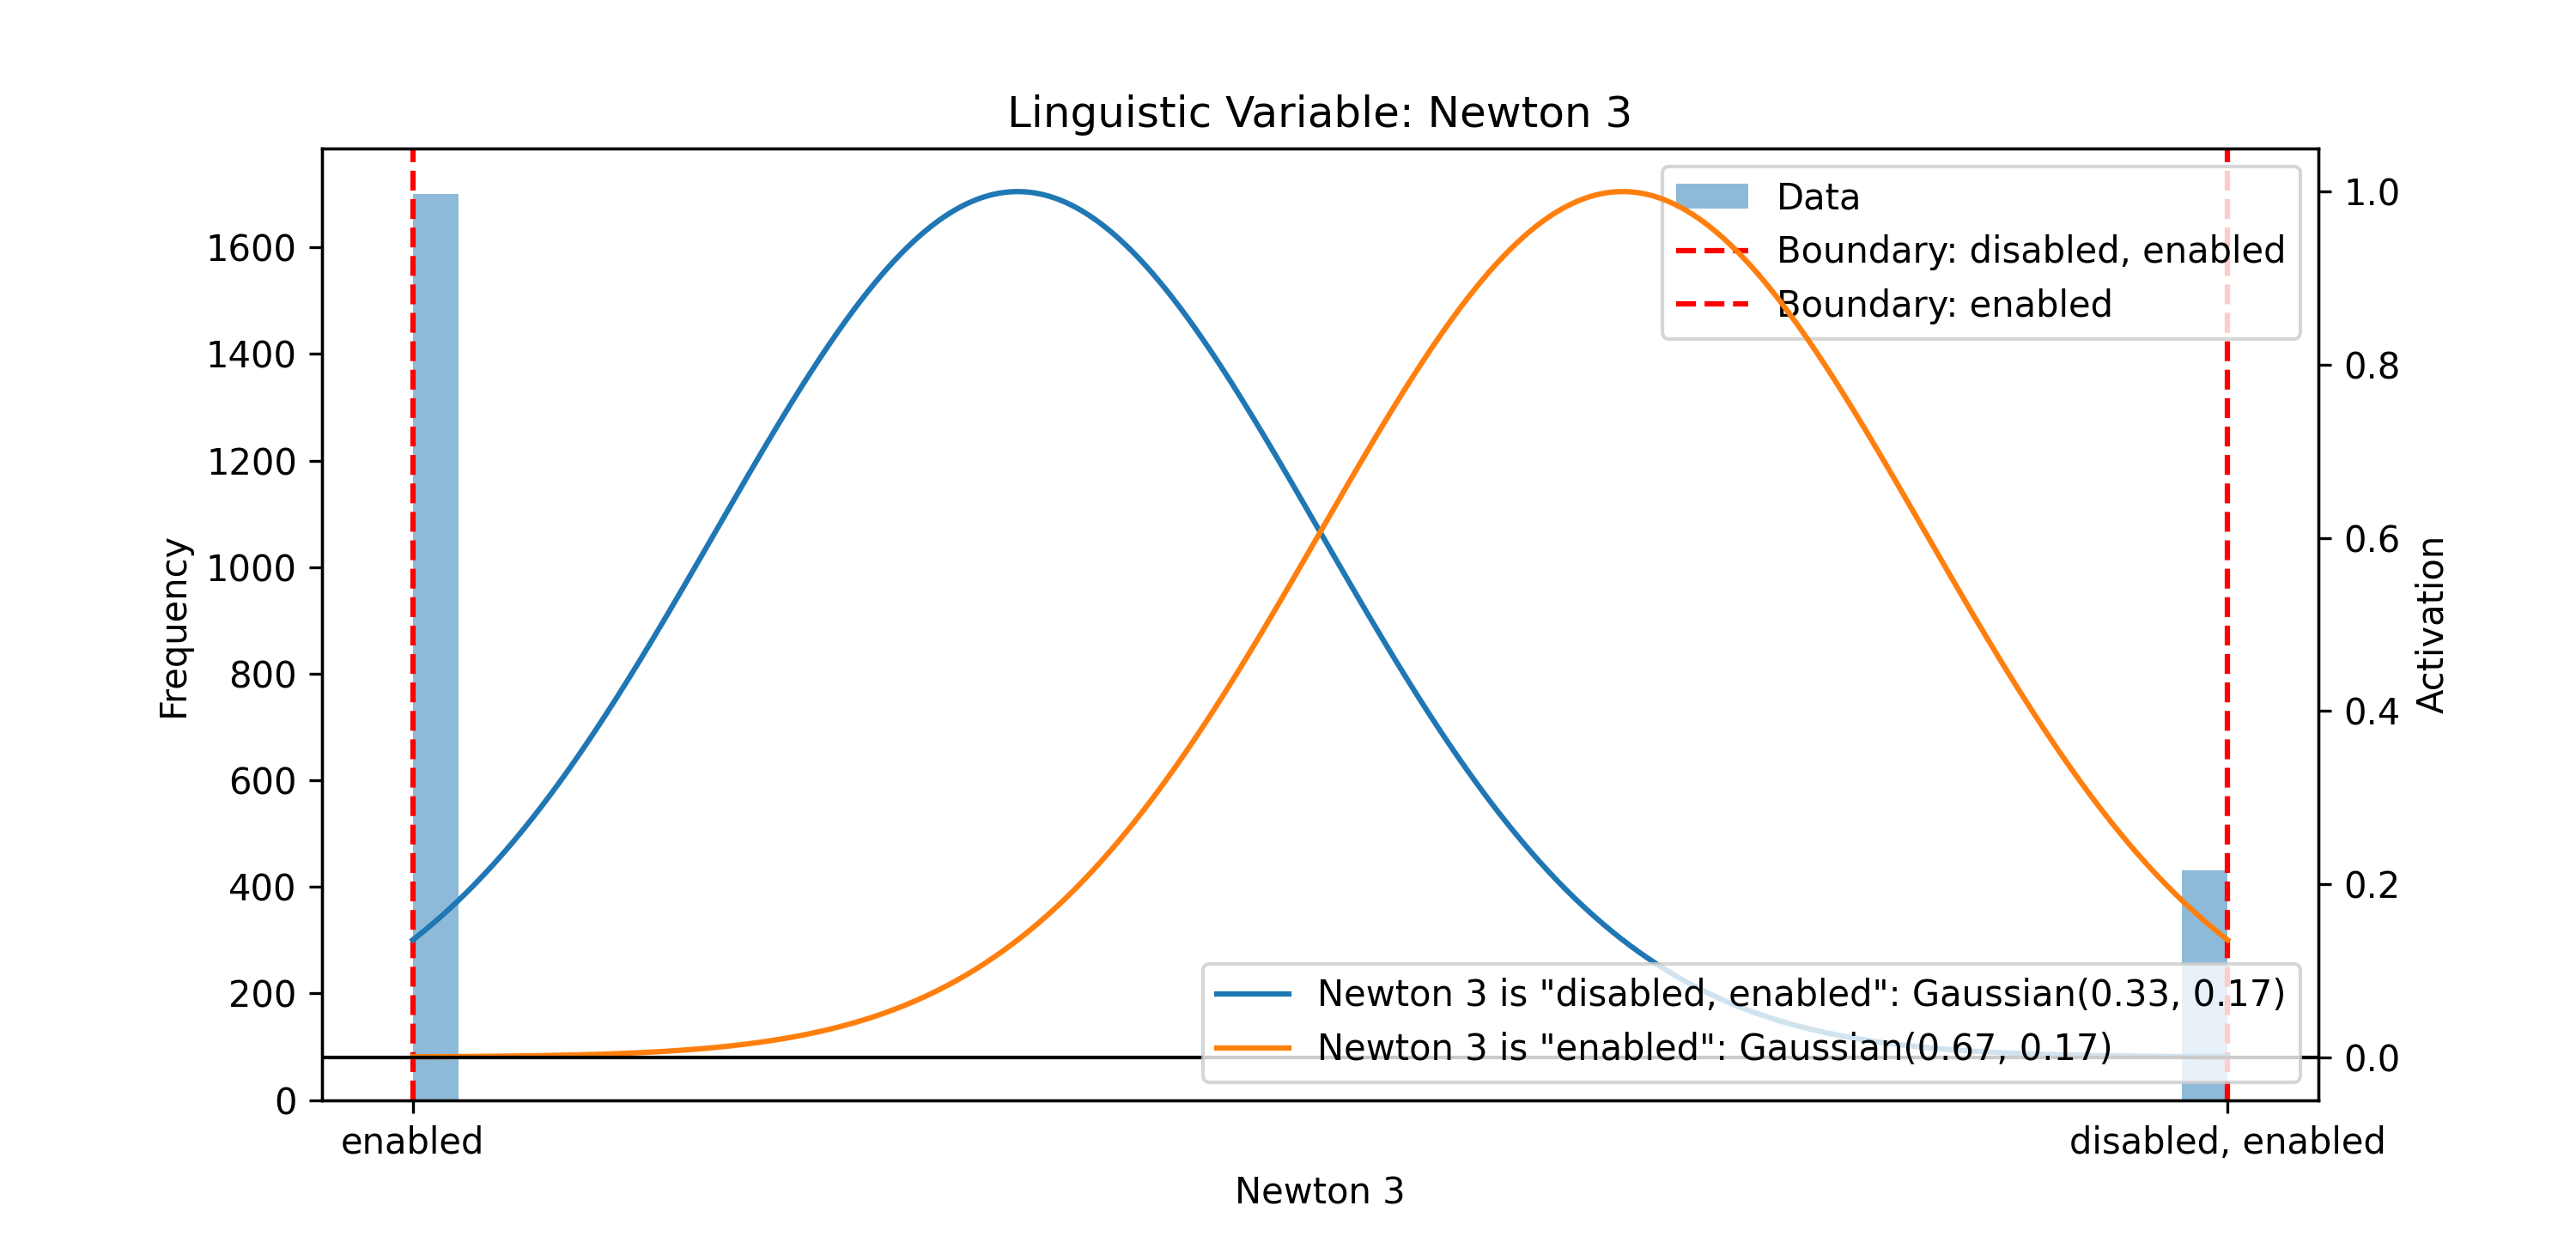
\includegraphics[width=\columnwidth,trim={1cm 0 1cm 1.35cm},clip]{figures/DataAnalytics/newton3_linguistic_variable.png}
        \caption[Linguistic variable for the Newton3 attribute]{
            This figure shows the linguistic variable for the Newton3 attribute. We see the two \texttt{gaussian} membership functions representing the two possible values for the Newton3 attribute.
        }
        \label{fig:newton3LinguisticVariable_component}
    \end{figure}
\end{multicols}

These linguistic variables and fuzzy rules are then used to create the fuzzy systems for the component tuning approach. The final Rule File for the component tuning approach can be looked up at \href{https://github.com/AutoPas/AutoPas/blob/f77f10f72c19a86d5471bce287ae3a4ae344c012/examples/md-flexible/input/fuzzyRulesComponents.frule}{\color{blue}\texttt{fuzzyRulesComponents.frule}}.


\subsection{Suitability Approach}

The suitability approach differs from the component tuning approach in that it tries to predict a configuration's numerical \emph{suitability} value under the current conditions. Therefore, each possible configuration is assigned a unique fuzzy system tailored to just evaluating this configuration. \autoref{fig:fuzzySystemSuitability} shows the structure of this approach.

To train the decision trees, we again use a classification-based approach with \texttt{terrible},\texttt{poor}, \texttt{bad}, \texttt{medium}, \texttt{ok}, \texttt{good}, and \texttt{excellent} as the possible linguistic terms corresponding to specific ranges of suitability values (see \autoref{fig:suitabilityClasses} for the exact placement). Conveniently, we can use $suitability= relative speed$, as the relative speed value already measures how well a configuration performs.

We create the training data for the decision trees by adding a new column to the aggregated training data containing the suitability class to which the numeric relative speed value mostly belongs. The final training data is shown in \autoref{tab:trainingDataSuitability}. After grouping the data by possible configurations, it is again possible to use these data points to train the decision trees and extract the fuzzy rules from them. Due to the grouping, each configuration receives its own fuzzy system with rules explicitly tailored to it. The resulting rules are shown in \autoref{tab:fuzzyRulesSuitability}.

\begin{figure}[H]
    \centering
    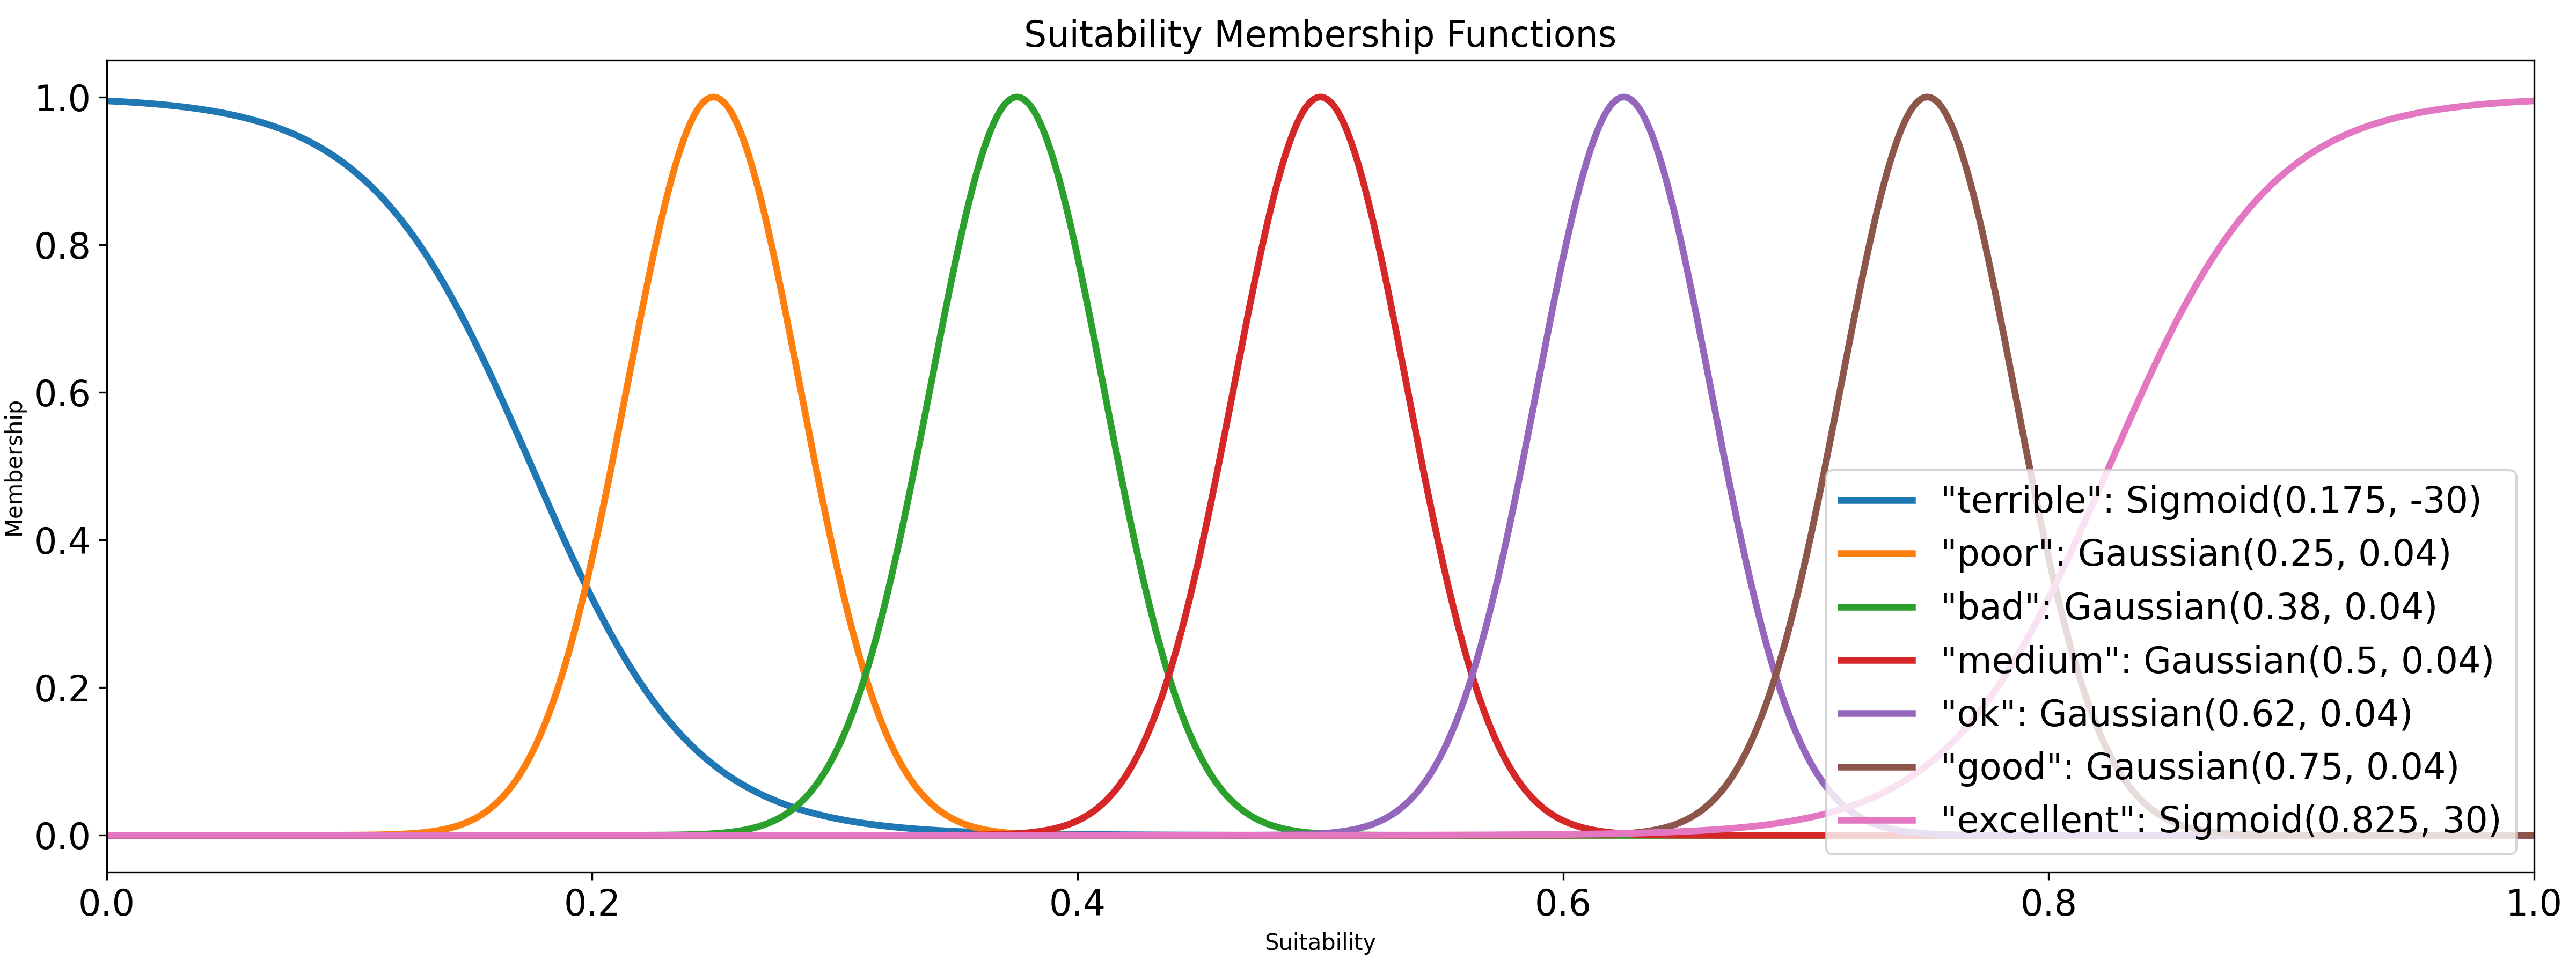
\includegraphics[width=\columnwidth,trim={0cm 0 0cm 0cm},clip]{figures/ProofOfConcepts/suitability_membership_functions.png}
    \caption[Linguistic variable for the Suitability attribute]{
        This figure shows the linguistic variable for the Suitability attribute. The domain between 0\% suitability and 100\% suitability is divided into 7 classes: \texttt{terrible}, \texttt{poor}, \texttt{bad}, \texttt{medium}, \texttt{ok}, \texttt{good}, and \texttt{excellent}. The central membership functions have a \texttt{gaussian} shape, while the outer ones have a \texttt{sigmoid} shape to capture the one-sided nature of those boundaries. The choice to use seven classes was made somewhat arbitrarily, with the intention to densely cover the range of suitability values.
    }
    \label{fig:suitabilityClasses}
\end{figure}

This approach makes it possible to use the \gls{cog} method for defuzzification, as the suitability values are ordinal. In order for the different fuzzy systems to be able to make individual choices, the Suitability values seen in \autoref{fig:suitabilityClasses} have to be duplicated for each configuration.

The resulting fuzzy systems can then be used to predict the suitability of all available configurations. The FuzzyTuningStrategy will combine all these predicted suitabilities and will only keep the configurations with the highest suitability values.

\newpage

\definecolor{LightRed}{rgb}{1,0.88,0.88}
\newcolumntype{u}{>{\columncolor{LightRed}}c}


\begin{table}[H]
    \centering
    \addtolength{\leftskip} {-3cm} % increase (absolute) value if needed
    \addtolength{\rightskip}{-3cm}
    \tiny
    \def\arraystretch{2.5}
    \begin{tabular}{|c|c|c|c|c|c|c|c|c|c|u|}
        \cline{1-9}
        \multicolumn{3}{|c|}{ \textbf{ParticlesPerCell}} & \multicolumn{3}{c|}{\textbf{Miscellaneous}} & \multicolumn{3}{c|}{\textbf{Configuration }}                                                                                                                                                            \\
        \hline
        \textbf{avg}                                     & \textbf{max}                                & \textbf{stddev}                              & \tabularCenterstack{c}{\textbf{homo-}                                                                                                                    \\ \textbf{genity}} & \tabularCenterstack{c}{\textbf{max-} \\ \textbf{density}} & \textbf{threads} & \tabularCenterstack{c}{\textbf{Container} \\ \textbf{DataLayout}}& \textbf{Traversal} & \textbf{Newton3}& \textbf{Relative speed}  & \textbf{Suitability}  \  \\
        \hline
        0.905                                            & 15                                          & 0.012                                        & 0.035                                 & 0.531  & 1      & LinkedCells\_AoS                              & lc sliced    & enabled  & 0.450  & "bad”       \\
        \hline
        0.944                                            & 25                                          & 0.012                                        & 0.083                                 & 0.691  & 28     & \tabularCenterstack{c}VerletClusterLists\_AoS & vcl\_c06     & disabled & 0.319  & "poor"      \\
        \hline
        0.944                                            & 20                                          & 0.012                                        & 0.079                                 & 0.041  & 12     & LinkedCell\_SoA                               & vlc\_ sliced & enabled  & 0.989  & "excellent" \\
        \hline
        \vdots                                           & \vdots                                      & \vdots                                       & \vdots                                & \vdots & \vdots & \vdots                                        & \vdots       & \vdots   & \vdots & \vdots      \\
        \hline
    \end{tabular}
    \caption[Training data for the Suitability Approach]{Training data for the Suitability Approach. The dataset contains the LiveInfoData of the simulation, the current configuration, the relative speed, and the suitability values of the configuration. Each row represents a different configuration evaluated in a tuning phase.}
    \label{tab:trainingDataSuitability}
\end{table}





\begin{table}[H]
    \footnotesize
    \centering
    \addtolength{\leftskip} {-3cm} % increase (absolute) value if needed
    \addtolength{\rightskip}{-3cm}

    \begin{tabular}{|c|c|c|c|g|}
        \multicolumn{4}{c}{\large{\textbf{Antecedent}}} & \multicolumn{1}{c}{\large{\textbf{Consequent}    }}                                                                                                                                  \\
        \hline
        \textbf{avgParticlesPC}                         & \textbf{homogeneity}                                & \textbf{particlesPCStdDev} & \textbf{threadCount}                              & \tabularCenterstack{c} { \textbf{Suitability} \\ \textbf{ LinkedCells\_AoS\_lc\_c01\_disabled}} \\

        \hline
                                                        & \texttt{lower than 0.084}                           & \texttt{higher than 0.029} & \texttt{higher than 26.0 }                        & "medium"                                      \\
        \hline
                                                        & \texttt{higher than 0.084}                          & \texttt{higher than 0.029} & \texttt{higher than 26.0 }                        & "bad"                                         \\
        \hline
                                                        &                                                     & \texttt{higher than 0.02}  & \texttt{lower than 2.5	 }                          & "poor"                                        \\

        \hline
        \vdots                                          & \vdots                                              & \vdots                     & \vdots                                            & \vdots                                        \\
        \hline

        \multicolumn{5}{c}{ }                                                                                                                                                                                                                  \\


        \multicolumn{4}{c}{\large{\textbf{Antecedent}}} & \multicolumn{1}{c}{\large{\textbf{Consequent}    }}                                                                                                                                  \\

        \hline
        \textbf{maxParticlesPerCell}                    & \textbf{homogeneity}                                & \textbf{particlesPCStdDev} & \textbf{threadCount}                              & \tabularCenterstack{c} { \textbf{Suitability} \\\textbf{ LinkedCells\_AoS\_lc\_c04\_disabled}}\\

        \hline
        \texttt{higher than 18.5	}                       & \texttt{lower than 0.082}                           &                            & \tabularCenterstack{c} {\texttt{higher than 18.0}                                                 \\ $\land$ \texttt{ lower than 26.0}} & "medium" \\

        \hline
        \texttt{higher than 18.5	}                       & \texttt{higher than 0.082}                          &                            & \tabularCenterstack{c} {\texttt{higher than 18.0}                                                 \\ $\land$ \texttt{ lower than 26.0}} & "bad" \\
        \hline


        \vdots                                          & \vdots                                              & \vdots                     & \vdots                                            & \vdots                                        \\

        \hline
        \multicolumn{2}{c}{}                            & \multicolumn{1}{c}{\Huge{\vdots   }}                                                                                                                                                 \\
    \end{tabular}

    \caption[Extracted fuzzy rules from the decision trees for the Suitability Approach]{Some extracted fuzzy rules from the decision trees for the Suitability Approach. The rules are grouped by the configuration they predict. The first row is read as:
        \footnotesize{$\text{IF} \;   (\text{homogeneity} = \text{lower than 0.084})   \land (\text{particlesPerCellStdDev} = \text{higher than 0.029})   \land (\text{threadCount} = \text{higher than 26.0}) \; \text{THEN} \; (\text{Suitability LinkedCells\_AoS\_lc\_c01\_disabled} = \text{"medium"})$}}
    \label{tab:fuzzyRulesSuitability}
\end{table}

The full Rule File for the suitability approach can be looked up at \href{https://github.com/AutoPas/AutoPas/blob/f77f10f72c19a86d5471bce287ae3a4ae344c012/examples/md-flexible/input/fuzzyRulesSuitability.frule}{\color{blue}\texttt{fuzzyRulesSuitability.frule}}.